%%%  کلاس AUTthesis، نسخه آبان 1397
%%%   دانشگاه صنعتی امیرکبیر                 http://www.aut.ac.ir
%%%  تالار گفتگوی پارسی‌لاتک،       http://forum.parsilatex.com
%%%   آپدیت شده در آبان 95
%%%   پشتیبانی و راهنمایی          badali_farhad@yahoo.com
%%%
%%%   بازبینی و اصلاح شده در آبان ماه 1397
%%%  Tested via TeXstudio in TeXlive 2014-2018.
%%%

%-----------------------------------------------------------------------------------------------------
%        روش اجرا.: 2 بار F1 ، 2 بار  F11(به منظور تولید مراجع) ، دوبار Ctrl+Alt+I (به منظور تولید نمایه) و دو بار F1 -------> مشاهده Pdf
%%%%%%%%%%%%%%%%%%%%%%%%%%%%%%%%%%%%%%%%%%%%%%%%%%%%%%
%   TeXstudio as your IDE
%%  برای compile در TeXstudio تنها کافی است منوی Options->Configure TeXstudio را زده و در پنجره Configure TeXstudio در بخش Build گزینه Default Compiler را به XeLaTeX تغییر دهید. سند شما به راحتی compile خواهد شد.
%   F1 & F5 : Build & view
%   F6      : Compile
%   F7      : View
%   --------------
%%%%%%%%%%%%%%%%%%%%%%%%%%%%%%%%%%%%%%%%%%%%%%%%%%%%%%
%        اگر قصد نوشتن رساله دکتری را دارید، در خط زیر به جای msc،
%      کلمه phd را قرار دهید. کلیه تنظیمات لازم، به طور خودکار، اعمال می‌شود.
%%% !TEX TS-program = XeLaTeX

\documentclass[oneside,bsc,12pt]{AUTthesis}
\usepackage{xcolor}
\usepackage{listings}
\usepackage{minted}
\definecolor{mGreen}{rgb}{0,0.6,0}
\definecolor{mGray}{rgb}{0.5,0.5,0.5}
\definecolor{mPurple}{rgb}{0.58,0,0.82}
\definecolor{backgroundColour}{rgb}{0.95,0.95,0.92}

\lstdefinestyle{CStyle}{
    backgroundcolor=\color{backgroundColour},   
    commentstyle=\color{mGreen},
    keywordstyle=\color{magenta},
    numberstyle=\tiny\color{mGray},
    stringstyle=\color{mPurple},
    basicstyle=\footnotesize,
    breakatwhitespace=false,         
    breaklines=true,                 
    captionpos=b,                    
    keepspaces=true,                 
    numbers=left,                    
    numbersep=5pt,                  
    showspaces=false,                
    showstringspaces=false,
    showtabs=false,                  
    tabsize=2,
    language=C
}

%       فایل commands.tex را حتماً به دقت مطالعه کنید؛ چون دستورات مربوط به فراخوانی بسته زی‌پرشین 
%       و دیگر بسته‌ها و ... در این فایل قرار دارد و بهتر است که با نحوه استفاده از آنها آشنا شوید. توجه شود برای نسخه نهایی پایان‌نامه حتماً hyperref را 
%        غیرفعال کنید.


% در این فایل، دستورها و تنظیمات مورد نیاز، آورده شده است.
%-------------------------------------------------------------------------------------------------------------------
% در ورژن جدید زی‌پرشین برای تایپ متن‌های ریاضی، این سه بسته، حتماً باید فراخوانی شود.
\usepackage{amsthm,amssymb,amsmath,amsfonts}
% بسته‌ای برای تنطیم حاشیه‌های بالا، پایین، چپ و راست صفحه
\usepackage[top=30mm, bottom=30mm, left=25mm, right=30mm]{geometry}
% بسته‌‌ای برای ظاهر شدن شکل‌ها و تصاویر متن
\usepackage{graphicx}
\usepackage{color}
%بسته‌ای برای تنظیم فاصله عمودی خط‌های متن
\usepackage{setspace}
\usepackage{titletoc}
\usepackage{tocloft}
%با فعال کردن بسته زیر فوت‌نوت‌ها در هر صفحه ریست می‌شوند. حالت پیش‌فرض آن ریست شدن در هر فصل می‌باشد.
%\usepackage[perpage]{footmisc}
\usepackage{enumitem}
%\usepackage{titlesec}
% بسته‌ و دستوراتی برای ایجاد لینک‌های رنگی با امکان جهش
\usepackage[pagebackref=false,colorlinks,linkcolor=blue,citecolor=red]{hyperref}
\usepackage[nameinlink]{cleveref}%capitalize,,noabbrev
 \AtBeginDocument{%
    \crefname{equation}{برابری}{equations}%
    \crefname{chapter}{فصل}{chapters}%
    \crefname{section}{بخش}{sections}%
    \crefname{appendix}{پیوست}{appendices}%
    \crefname{enumi}{مورد}{items}%
    \crefname{footnote}{زیرنویس}{footnotes}%
    \crefname{figure}{شکل}{figures}%
    \crefname{table}{جدول}{tables}%
    \crefname{theorem}{قضیه}{theorems}%
    \crefname{lemma}{لم}{lemmas}%
    \crefname{corollary}{نتیجه}{corollaries}%
    \crefname{proposition}{گزاره}{propositions}%
    \crefname{definition}{تعریف}{definitions}%
    \crefname{result}{نتیجه}{results}%
    \crefname{example}{مثال}{examples}%
    \crefname{remark}{نکته}{remarks}%
    \crefname{note}{یادداشت}{notes}%
}
% چنانچه قصد پرینت گرفتن نوشته خود را دارید، خط بالا را غیرفعال و  از دستور زیر استفاده کنید چون در صورت استفاده از دستور زیر‌‌، 
% لینک‌ها به رنگ سیاه ظاهر خواهند شد که برای پرینت گرفتن، مناسب‌تر است
%\usepackage[pagebackref=false]{hyperref}
% بسته‌ لازم برای تنظیم سربرگ‌ها
\usepackage{fancyhdr}
% بسته‌ای برای ظاهر شدن «مراجع»  در فهرست مطالب
\usepackage[nottoc]{tocbibind}
% دستورات مربوط به ایجاد نمایه
\usepackage{makeidx,multicol}
\setlength{\columnsep}{1.5cm}

%%%%%%%%%%%%%%%%%%%%%%%%%%
\usepackage{verbatim}
\makeindex
\usepackage{sectsty}
% فراخوانی بسته زی‌پرشین و تعریف قلم فارسی و انگلیسی
\usepackage{xepersian}%[extrafootnotefeatures]
\SepMark{-}
%حتماً از تک لایو 2014 استفاده کنید.
\settextfont[Scale=1.2]{B-NAZANIN.TTF}
\setlatintextfont{times.ttf}
\renewcommand{\labelitemi}{$\bullet$}
%%%%%%%%%%%%%%%%%%%%%%%%%%
% چنانچه می‌خواهید اعداد در فرمول‌ها، انگلیسی باشد، خط زیر را غیرفعال کنید.
%در غیر اینصورت حتماً فونت PGaramond را نصب کنید.
%\setdigitfont[Scale=1.1]{PGaramond.ttf}%%Yas
%%%%%%%%%%%%%%%%%%%%%%%%%%
% تعریف قلم‌های فارسی اضافی برای استفاده در بعضی از قسمت‌های متن
\defpersianfont\nastaliq[Scale=2]{IranNastaliq.ttf}
\defpersianfont\chapternumber[Scale=3]{B-NAZANIN.TTF}
\defpersianfont\nas[Scale=1.5]{B-NAZANIN.TTF}
%\chapterfont{\centering}%
%%%%%%%%%%%%%%%%%%%%%%%%%%
% دستوری برای تغییر نام کلمه «اثبات» به «برهان»
\renewcommand\proofname{\textbf{برهان}}

% دستوری برای تغییر نام کلمه «کتاب‌نامه» به «منابع و مراجع«
\renewcommand{\bibname}{منابع و مراجع}


% Headings for every page of ToC, LoF and Lot
\setlength{\cftbeforetoctitleskip}{-1.2em}
\setlength{\cftbeforelottitleskip}{-1.2em}
\setlength{\cftbeforeloftitleskip}{-1.2em}
\setlength{\cftaftertoctitleskip}{-1em}
\setlength{\cftafterlottitleskip}{-1em}
\setlength{\cftafterloftitleskip}{-1em}
%%\makeatletter
%%%%\renewcommand{\l@chapter}{\@dottedtocline{1}{1em\bfseries}{1em}}
%%%%\renewcommand{\l@section}{\@dottedtocline{2}{2em}{2em}}
%%%%\renewcommand{\l@subsection}{\@dottedtocline{3}{3em}{3em}}
%%%%\renewcommand{\l@subsubsection}{\@dottedtocline{4}{4em}{4em}}
%%%%\makeatother


\newcommand\tocheading{\par عنوان\hfill صفحه \par}
\newcommand\lofheading{\hspace*{.5cm}\figurename\hfill صفحه \par}
\newcommand\lotheading{\hspace*{.5cm}\tablename\hfill صفحه \par}

\renewcommand{\cftchapleader}{\cftdotfill{\cftdotsep}}
\renewcommand{\cfttoctitlefont}{\hspace*{\fill}\LARGE\bfseries}%\Large
\renewcommand{\cftaftertoctitle}{\hspace*{\fill}}
\renewcommand{\cftlottitlefont}{\hspace*{\fill}\LARGE\bfseries}%\Large
\renewcommand{\cftafterlottitle}{\hspace*{\fill}}
\renewcommand{\cftloftitlefont}{\hspace*{\fill}\LARGE\bfseries}
\renewcommand{\cftafterloftitle}{\hspace*{\fill}}

%%%%%%%%%%%%%%%%%%%%%%%%%%
% تعریف و نحوه ظاهر شدن عنوان قضیه‌ها، تعریف‌ها، مثال‌ها و ...
%برای شماره گذاری سه تایی قضیه ها
\theoremstyle{definition}
\newtheorem{definition}{تعریف}[section]
\newtheorem{remark}[definition]{نکته}
\newtheorem{note}[definition]{یادداشت}
\newtheorem{example}[definition]{نمونه}
\newtheorem{question}[definition]{سوال}
\newtheorem{remember}[definition]{یاداوری}
\theoremstyle{theorem}
\newtheorem{theorem}[definition]{قضیه}
\newtheorem{lemma}[definition]{لم}
\newtheorem{proposition}[definition]{گزاره}
\newtheorem{corollary}[definition]{نتیجه}
%%%%%%%%%%%%%%%%%%%%%%%%
%%%%%%%%%%%%%%%%%%%
%%% برای شماره گذاری چهارتایی قضیه ها و ...
%%\newtheorem{definition1}[subsubsection]{تعریف}
%%\newtheorem{theorem1}[subsubsection]{قضیه}
%%\newtheorem{lemma1}[subsubsection]{لم}
%%\newtheorem{proposition1}[subsubsection]{گزاره}
%%\newtheorem{corollary1}[subsubsection]{نتیجه}
%%\newtheorem{remark1}[subsubsection]{نکته}
%%\newtheorem{example1}[subsubsection]{مثال}
%%\newtheorem{question1}[subsubsection]{سوال}

%%%%%%%%%%%%%%%%%%%%%%%%%%%%

% دستورهایی برای سفارشی کردن صفحات اول فصل‌ها
\makeatletter
\newcommand\mycustomraggedright{%
 \if@RTL\raggedleft%
 \else\raggedright%
 \fi}
\def\@makechapterhead#1{%
\thispagestyle{style1}
\vspace*{20\p@}%
{\parindent \z@ \mycustomraggedright
\ifnum \c@secnumdepth >\m@ne
\if@mainmatter

\bfseries{\Huge \@chapapp}\small\space {\chapternumber\thechapter}
\par\nobreak
\vskip 0\p@
\fi
\fi
\interlinepenalty\@M 
\Huge \bfseries #1\par\nobreak
\vskip 120\p@

}

%\thispagestyle{empty}
\newpage}
\bidi@patchcmd{\@makechapterhead}{\thechapter}{\tartibi{chapter}}{}{}
\bidi@patchcmd{\chaptermark}{\thechapter}{\tartibi{chapter}}{}{}
\makeatother

\pagestyle{fancy}
\renewcommand{\chaptermark}[1]{\markboth{\chaptername~\tartibi{chapter}: #1}{}}

\fancypagestyle{style1}{
\fancyhf{} 
\fancyfoot[c]{\thepage}
\fancyhead[R]{\leftmark}%
\renewcommand{\headrulewidth}{1.2pt}
}


\fancypagestyle{style2}{
\fancyhf{}
\fancyhead[R]{چکیده}
\fancyfoot[C]{\thepage{}}
\renewcommand{\headrulewidth}{1.2pt}
}

\fancypagestyle{style3}{%
  \fancyhf{}%
  \fancyhead[R]{فهرست نمادها}
  \fancyfoot[C]{\thepage}%
  \renewcommand{\headrulewidth}{1.2pt}%
}

\fancypagestyle{style4}{%
  \fancyhf{}%
  \fancyhead[R]{فهرست جداول}
  \fancyfoot[C]{\thepage}%
  \renewcommand{\headrulewidth}{1.2pt}%
}

\fancypagestyle{style5}{%
  \fancyhf{}%
  \fancyhead[R]{فهرست اشکال}
  \fancyfoot[C]{\thepage}%
  \renewcommand{\headrulewidth}{1.2pt}%
}

\fancypagestyle{style6}{%
  \fancyhf{}%
  \fancyhead[R]{فهرست مطالب}
  \fancyfoot[C]{\thepage}%
  \renewcommand{\headrulewidth}{1.2pt}%
}

\fancypagestyle{style7}{%
  \fancyhf{}%
  \fancyhead[R]{نمایه}
  \fancyfoot[C]{\thepage}%
  \renewcommand{\headrulewidth}{1.2pt}%
}

\fancypagestyle{style8}{%
  \fancyhf{}%
  \fancyhead[R]{منابع و مراجع}
  \fancyfoot[C]{\thepage}%
  \renewcommand{\headrulewidth}{1.2pt}%
}
\fancypagestyle{style9}{%
  \fancyhf{}%
  \fancyhead[R]{واژه‌نامه‌ی فارسی به انگلیسی}
  \fancyfoot[C]{\thepage}%
  \renewcommand{\headrulewidth}{1.2pt}%
}
%


%دستور حذف نام لیست تصاویر و لیست جداول از فهرست مطالب
\newcommand*{\BeginNoToc}{%
  \addtocontents{toc}{%
    \edef\protect\SavedTocDepth{\protect\the\protect\value{tocdepth}}%
  }%
  \addtocontents{toc}{%
    \protect\setcounter{tocdepth}{-10}%
  }%
}
\newcommand*{\EndNoToc}{%
  \addtocontents{toc}{%
    \protect\setcounter{tocdepth}{\protect\SavedTocDepth}%
  }%
}
\newcounter{savepage}
\renewcommand{\listfigurename}{فهرست اشکال}
\renewcommand{\listtablename}{فهرست جداول}
%\renewcommand\cftsecleader{\cftdotfill{\cftdotsep}}
%%%%%%%%%%%%%%%%%%%%%%%%%%%%%
%%%%%%%%%%%%%%%%%%%%%%%%%%%%

\begin{document}
\baselineskip=.75cm
\linespread{1.75}
%% -!TEX root = AUTthesis.tex
% در این فایل، عنوان پایان‌نامه، مشخصات خود، متن تقدیمی‌، ستایش، سپاس‌گزاری و چکیده پایان‌نامه را به فارسی، وارد کنید.
% توجه داشته باشید که جدول حاوی مشخصات پروژه/پایان‌نامه/رساله و همچنین، مشخصات داخل آن، به طور خودکار، درج می‌شود.
%%%%%%%%%%%%%%%%%%%%%%%%%%%%%%%%%%%%
% دانشکده، آموزشکده و یا پژوهشکده  خود را وارد کنید
\faculty{دانشکده مهندسی کامپیوتر}
% گرایش و گروه آموزشی خود را وارد کنید
 \department{}
% عنوان پایان‌نامه را وارد کنید
\fatitle{
دستور کار آزمایشگاه ریزپردازنده}
%\secondsupervisor{استاد راهنمای دوم}
% نام استاد(دان) مشاور را وارد کنید. چنانچه استاد مشاور ندارید، دستور پایین را غیرفعال کنید.
% \firstadvisor{دکتر حامد فربه}
%\secondadvisor{استاد مشاور دوم}
% نام نویسنده را وارد کنید
\name{امیرحسین پولاد، علی انصاری، ریحانه باقری، محمدحسین صباغی، امید خباز قانع، امیررضا طربخواه، علیرضا جلوخانی}
% نام خانوادگی نویسنده را وارد کنید
\surname{}
%%%%%%%%%%%%%%%%%%%%%%%%%%%%%%%%%%
\thesisdate{زمستان ۱۴۰۱}


\AUTtitle
%%%%%%%%%%%%%%%%%%%%%%%%%%%%%%%%%%
\vspace*{7cm}
\thispagestyle{empty}
\begin{center}

\includegraphics[height=5cm,width=12cm]{besm}
\end{center}
% دستور زیر برای شماره گذاری صفحات قبل از فصل اول با حروف ابجد است.
\pagenumbering{alph}
%-----------------------------------------------------------------------------
% فایل زیر دستورات مربوط به نمایش صفحات فهرست مطالب- فهرست اشکال و جداول است.
%{\pagestyle{style2}
%\tableofcontents}\newpage
%
%\listoffigures
\cleardoublepage
\pagestyle{style6}
\tableofcontents
\pagestyle{style6}
\cleardoublepage
%اگر لیست تصاویر و لیست جداول ندارید ، کدهای زیر را با گذاشتن % در ابتدای آنها، غیرفعال کنید.
%\BeginNoToc
%============
%\addtocontents{lof}{\lofheading}% add heading to the first page in LoF
%\pagestyle{style5}
%\listoffigures
%\thispagestyle{style5}
%\cleardoublepage
%============
% \addtocontents{lot}{\lotheading}% add heading to the first page in LoT
% \thispagestyle{style4}
% \listoftables
% \thispagestyle{style4}
%============
%\cleardoublepage
%
%\cleardoublepage
%\setcounter{savepage}{\arabic{page}}
%\mainmatter
%\addtocontents{toc}{\tocheading}% add heading to the first page in ToC, after frontmatter entries
%\EndNoToc
% در صورت تمایل می‌توانید با فعال کردن دستور بالا، لیست تصاویر را به  پایان‌نامه خود اضافه کنید.
%-------------------------------------------------------------------------symbols(فهرست نمادها)
% وجود لیست نمادها الزامیست.(لطفاً نمادهای خود را جایگذین نمادهای پیش‌فرض کنید.)
%%%%%%%%%%%%%%

\pagenumbering{alph}
\setcounter{page}{\thesavepage}
%\setcounter{page}{6}
\vspace*{1cm}

\pagestyle{style3}
\thispagestyle{style3}
\newpage
%\pagestyle{style1}
%%%%%%%%%%%%%%%%%%%%%%%%%%%%%%%%%%%%


\pagenumbering{arabic}
\pagestyle{style1}
%--------------------------------------------------------------------------chapters(فصل ها)
\definecolor{bg}{rgb}{0.95,0.95,0.95}
\chapter{مقدمات و نکات امنیتی}
\section{مسائل مقدماتی در آزمایشگاه ریزپردازنده}

\subsection{قوانین آزمایشگاه ریزپردازنده}
به منظور افزایش کارایی درس آزمایشگاه ریزپردازنده، رعایت عدالت میان همه‌ی گروه های آزمایشگاه و آموزش حداکثری مطالب درس به صورت عمل، مدرسی و دانشجویان ملزم به رعایت نکات و قوانین زیر هستند:
\begin{enumerate}
    \item مدرسین و دانشجویان موظفند راس ساعت در کلاس حاضر شوند.
    \item غیبت در هیچ یک از جلسات آزمایشگاه مجاز نیست.
    \item آزمایش ها در گروه های دو نفره انجام می‌شوند.
    \item ارائه‌ی پیش گزارش به صورت انفرادی‌است و هر دانشجو موظف است برای هر آزمایش پیش‌گزارش آن را تهیه نماید. پیش‌گزارش شامل جواب سوال هایی که با رنگ قرمز در قسمت مقدمه‌ی هر آزمایش آمده می‌شود.
    \item نیازی به ارائه‌ی گزارش‌کار برای آزمایش ها نیست و تحویل خروجی صحیح به مدرس آزمایشگاه کفایت می‌کند.
\end{enumerate}

\subsection{آشنایی با بردبورد}

در دنیای سیستم های نهفته و مدار های الکترونیکی معمولا برای سریع تر شدن فرایند توسعه، ابتدا یک نمونه‌ی اولیه با بردبورد می‌سازند و بعد از توسعه‌ی محصول نهایی سراغ تهیه‌ی مدار چاپی و یا روش های دیگر می‌روند. ما نیز در آزمایشگاه ریزپردازنده آزمایش های گفته شده را با استفاده از بردبورد انجام می‌دهیم.
\begin{figure}[h]
    \centering
    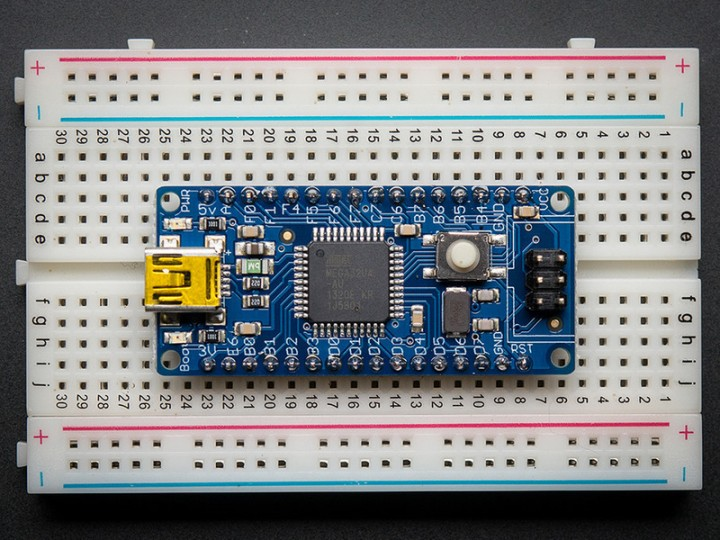
\includegraphics[width=6cm]{breadboard.png}
    \caption{تصویر یک بردبورد که روی آن یک میکروکنترلر قرار داده شده‌است.}
    \label{fig:breadboard}
\end{figure}

بردبورد در واقع یک مدار با اتصالات از پیش تعیین شده است، به طوری که سوراخ های میانی به صورت عمودی و سوراخ های دو ردیف بالا و پایین به صورت افقی به یکدیگر اتصال الکتریکی دارند. پیشنهاد می‌شود که از این دو ردیف برای اتصال مثبت و منفی منبع ولتاژ استفاده کنید. عمدتا در این درس مثبت و منفی از پین های \lr{5V} و \lr{GND} میکروکنترل تامین می‌شود اما می‌تواند به هر صورت دیگری نیز باشد. 

\subsection{آشنایی با بورد \lr{Arduino Uno}}

در این آزمایشگاه از بورد \lr{Arduino Uno} استفاده می‌کنیم. این بورد مبتنی بر میکروکنترلر \lr{ATmega328P} است که شامل ۱۴ پین خروجی و ورودی است که ۶ تا از آنها قابلیت خروجی \lr{PWM} و ۶ تا از آنها قابلیت خروجی آنالوگ دارند. همچنین این میکروکنترلر ۳۲ کیلوبایت حافظه‌ی فلش (که از آن ۰.۵ کیلوبایت برای برنامه‌ی بوتلودر استفاده شده) و ۲ کیلوبایت \lr{SRAM} و ۱ کیلوبایت حافظه‌ی \lr{EEPROM} دارد.
\lr{
\begin{center}
\begin{tabular}{ |c|c| } 
 \hline
 \lr{Microcontroller} & \lr{ATmega328P} \\ 
  \hline
 \lr{Operating Voltage} & \lr{5V} \\ 
  \hline
 \lr{Input Voltage (recommended)} & \lr{7-12V} \\ 
  \hline
 \lr{Input Voltage (limit)} & \lr{6-20V} \\ 
  \hline
 \lr{Digital I/O Pins} & \lr{14 (of which 6 provide PWM output)} \\ 
  \hline
 \lr{PWM Digital I/O Pins} & \lr{6} \\ 
  \hline
 \lr{Analog Input Pins} & \lr{6} \\ 
  \hline
 \lr{DC Current per I/O Pin} & \lr{20 mA} \\
  \hline
 \lr{DC Current for 3.3V Pin} & \lr{50mA} \\
  \hline
\lr{ Flash Memory} & \lr{32 KB (ATmega328P) of which 0.5 KB used by bootloader} \\ 
 \hline
 \lr{SRAM} & \lr{2 KB (ATmega328P)} \\ 
  \hline
 \lr{EEPROM} &  \lr{1 KB (ATmega328P)} \\
  \hline
 \lr{Clock Speed} &  \lr{16 MHz} \\ 
 \hline
\end{tabular}
\end{center}
}
\begin{figure}[h]
    \centering
    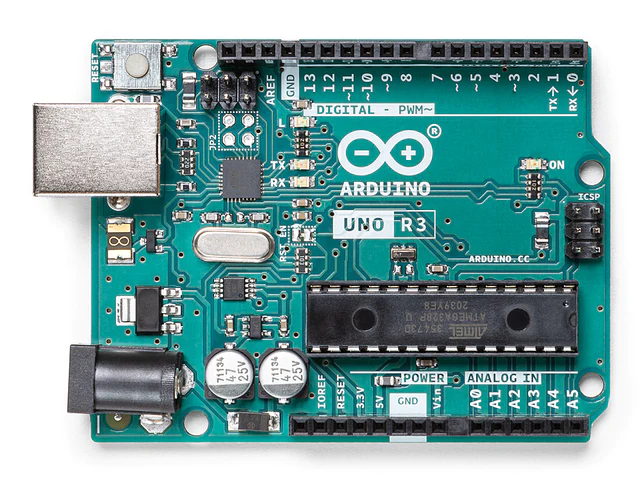
\includegraphics[width=8cm]{ArdUno.png}
    \caption{تصویری از بورد \lr{Arduino Uno}}
    \label{fig:arduno}
\end{figure}

\subsection{آشنایی با محیط \lr{Arduino IDE}}
بورد های آردوینو را می‌توان به راحتی با استفاده از برنامه‌ی \lr{Arduino IDE} برنامه ریزی کرد و نقطه قوت اصلی آن نسبت به پلتفرم های دیگر نیز همین سهولت در برنامه ریزی آنهاست. در ابتدا شما باید ابتدا این برنامه را از \href{https://www.arduino.cc/en/software}{این لینک} دریافت کرده و نصب کنید و سپس آن را اجرا کنید.
پس از اجرای برنامه با محیط زیر روبرو می‌شوید:

\begin{figure}[h]
    \centering
    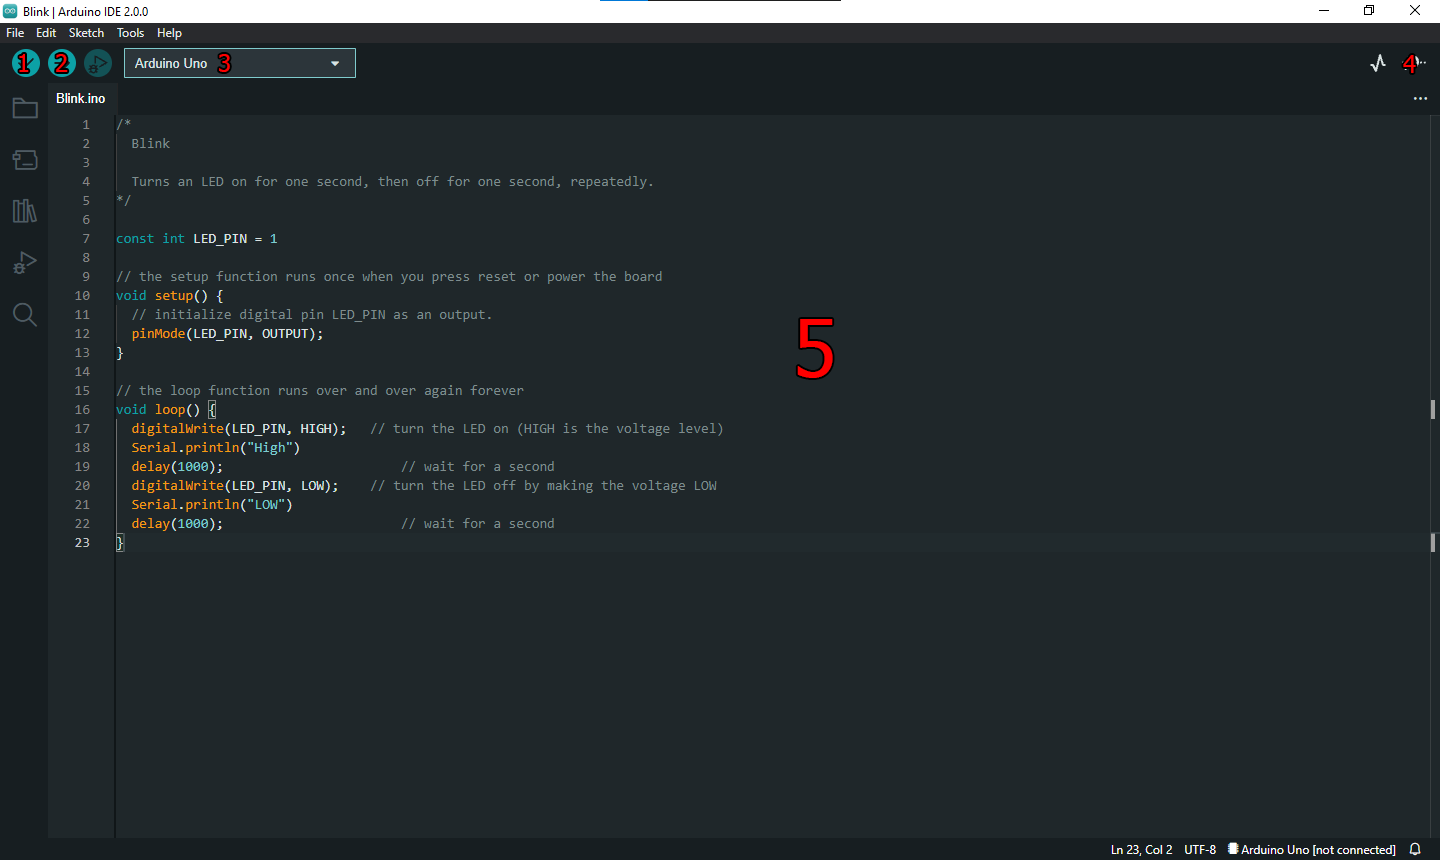
\includegraphics[width=16cm]{arduinoide1.png}
    \caption{تصویری از محیط \lr{Arduino IDE}}
    \label{fig:ardunoide}
\end{figure}

\begin{enumerate}
    \item کامپایل برنامه
    \item کامپایل برنامه و آپلود آن بر روی بورد
    \item انتخاب بورد
    \item سریال مانیتور
    \item ادیتور کد
\end{enumerate}

با این محیط در ویدیو های آموزشی که در اختیار شما قرار می‌گیرد بیشتر آشنا خواهیم شد.

\section{نکات امنیتی کار با قطعات الکترونیکی}

\subsection{دیود نوری}
دیود های نوری یک حداکثر جریان قابل تحمل دارند و اگر جریان عبور از آنها از یک مقدار معین بیشتر شود می‌سوزند. برای همین همواره از یک مقاومت سری حداقل ۱۰۰ اهمی برای محدود کردن جریان دیود استفاده می‌کنیم. در آزمایش اول بیشتر با نحوه‌ی محاسبه‌ی مقاومت مورد نیاز برای دیود های نوری آشنا می‌شویم.

\subsection{جریان خروجی از پین های میکروکنترلر}

پین های ورودی و خروجی میکروکنترلر ها محدودیت جریانی ۲۰ میلی‌آمپری دارند. توجه کنید و به هیچ وجه مداری نبندید که جریان خروجی از پین های میکروکنترلر از ۲۰ میلی‌آمپر بیشتر شوند. در غیر این صورت امکان خرابی قطعه وجود دارد و عواقب آن بر عهده‌ی خودتان است. برای اینکه مدار هایی با جریان عبوری بیشتر را توسط میکروکنترلر کنترل کنیم باید از ترانزیستور و یا رله استفاده کنیم که در آزمایش های آینده بیشتر با آن آشنا خواهیم شد.

\subsection{راهنمای پین های آردوینو}
\begin{figure}[h]
    \centering
    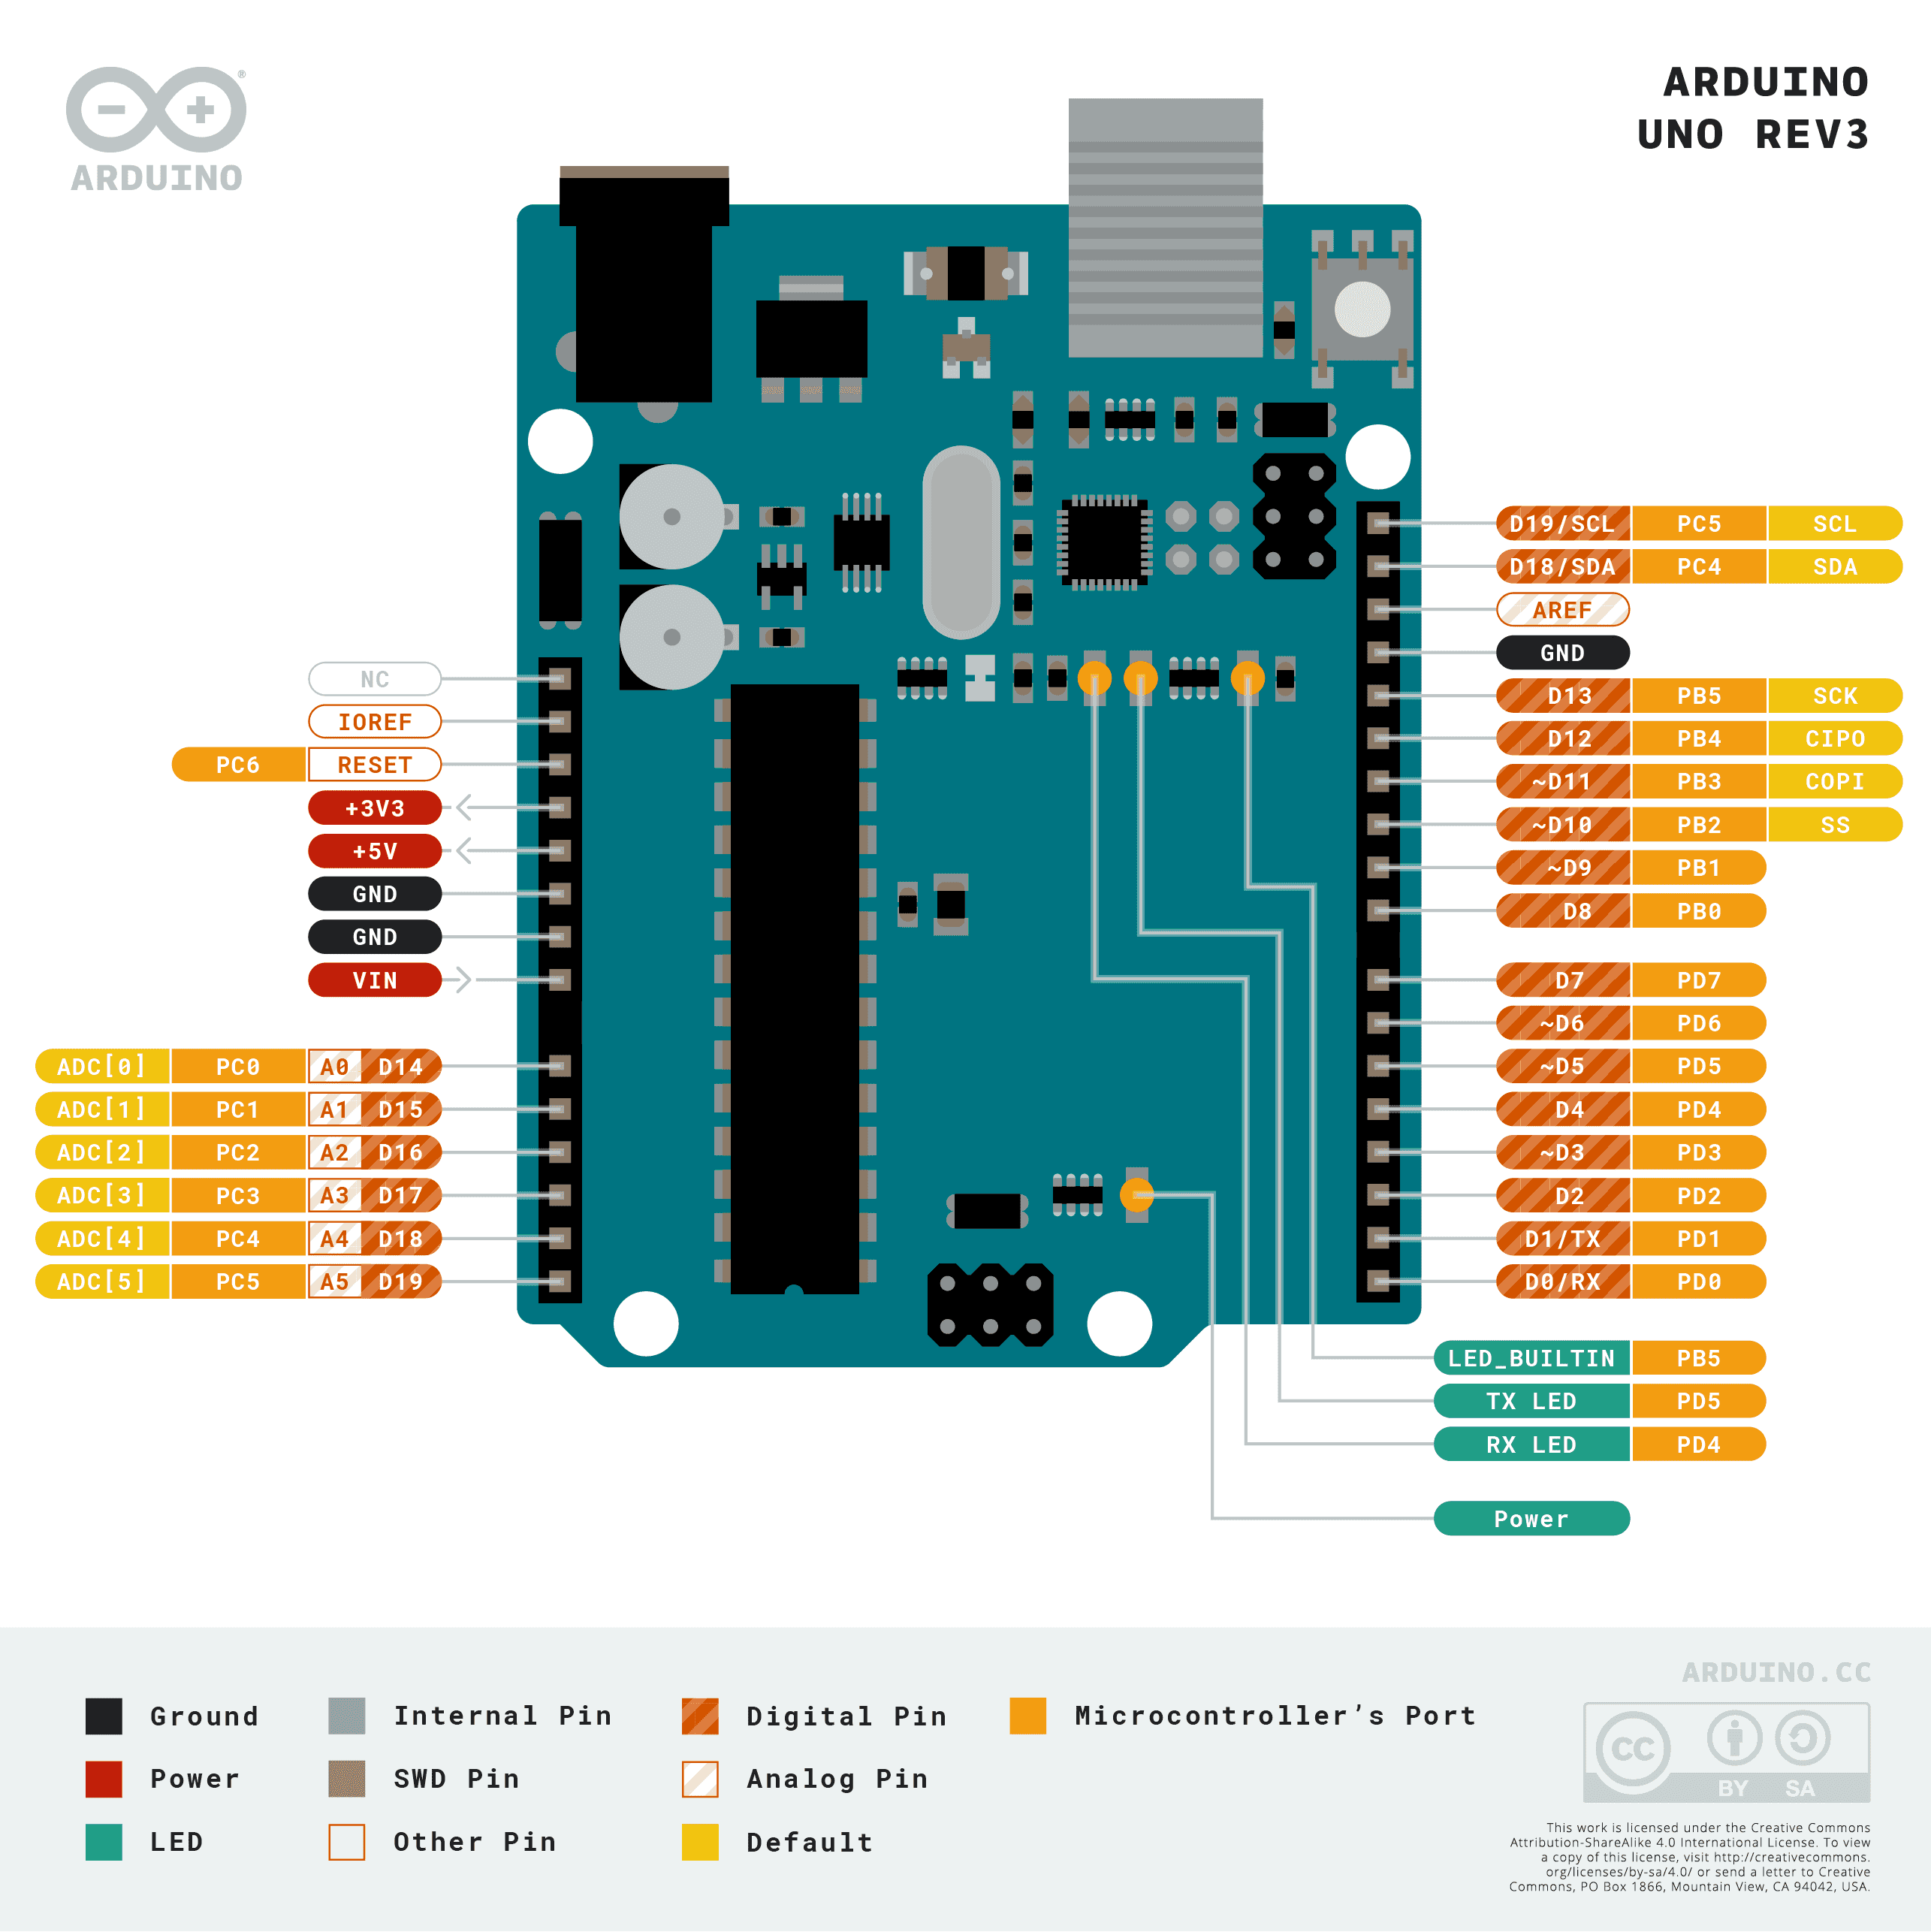
\includegraphics[width=16cm]{Pinout-UNO.png}
    \caption{راهنمای پین های آردوینو}
    \label{fig:ard_pinout}
\end{figure}

\
\section{دستور کار صفرم - تمرین کلاسی}

قبل از شروع آزمایش‌ها، نیاز است برخی مقدمات و مسائل در مورد ریزپردازنده‌های مورد استفاده و همچنین مدارهای الکریکی مرور شوند. برای این کار، در مورد مسائلی که گفته می‌شوند تحقیق کنید.

\subsection{آردوینو}
در این آزمایشگاه از میکروکنترلرهای سری آردوینو استفاده خواهیم کرد. در مورد میکروکنترلر‌های
\lr{Arduino Uno}،
\lr{Arduino Due}،
\lr{Arduino Nano} و 
\lr{Arduino Mega}
تحقیق کنید و برای هر کدام موارد زیر را پیدا کنید:

\begin{enumerate}
    \item مشخصات برد
    \item مشخصات ریزپردازنده استفاده شده
    \item ولتاژ کاری
    \item تعداد ورودی و خروجی آنالوگ و دیجیتال و \lr{PWM} و پاور
    \item جریان مجاز قابل عبور از هر پین
\end{enumerate}

\subsection{مدارهای الکتریکی}

از آنجا که کار با ریزپردازنده‌ها و مدارهای الکتریکی بسیار مرتبطند، دانش مقدماتی از مدارهای الکتریکی مورد نیاز است. در مورد موارد زیر تحقیق کنید:

\begin{enumerate}
    \item قانون اهم
    \item قانون‌های مداری کیرشهف
    \item نحوه کار بردبورد
    \item نحوه خواندن کد رنگی مقاومت
    \item نحوه بستن خازن و مقاومت به صورت سری یا موازی و فرمول‌های مقاومت و ظرفیت معادل
\end{enumerate}
\definecolor{bg}{rgb}{0.95,0.95,0.95}
\chapter{دستور کار آزمایش ها}

\section{کار با پایه های ورودی خروجی به روش های سرکشی و وقفه محور}

\subsection{اهداف آزمایش}
\begin{itemize}
    \item آشنایی با \lr{GPIO}
    \item آشنایی با روش های سرکشی و وقفه محور برای مدیریت \lr{Peripheral} های جانبی
    \item مقایسه‌ی دو روش سرکشی و وقفه محور
\end{itemize}

\subsection{قطعات مورد نیاز}

\begin{itemize}
    \item بورد \lr{Arduino Uno}
    \item دیود نورانی \lr{LED}
    \item کلید \lr{Switch}
    \item مقاومت ۲۲۰ اهم
    \item مقاومت ۱۰ هزار اهم
\end{itemize}
\pagebreak

\subsection{مقدمه}

\begin{nas} دو تابع اصلی در برنامه‌نویسی آردوینو \end{nas}
\newline
محیط آردوینو برای راحت تر شدن برنامه‌نویسی ۲ تابع مهم در اختیار ما می‌گذارد. نام این دو تابع \lr{begin} و \lr{loop} است.
\newline
\textcolor{red}{\begin{nas}سوال: \end{nas}}
در مورد این دو تابع تحقیق کنید و بنویسید که هر کدام در چه زمانی اجرا می‌شوند.

\newline
\begin{nas}دیود نوری
\end{nas}
\newline
دیود های نوری نوعی دیود هستند که هنگام عبور جریان از پایانه‌ی مثبت به پایانه‌ی منفی آنها، از خود نور ساتع می‌کنند. خواص الکتریکی دیود های نوری مشابه با دیود های دیگر است. این یعنی می‌توان یک دیود نوری روشن را به صورت یک منبع ولتاژ مدل سازی کرد. همچنین جریان عبوی از دیود های نوری دارای یک محدودیت است و اگر جریان بیشتر شود دیود نوری می‌سوزد و به همین دلیل باید در مدار شامل دیود نوری یک مقاومت حدودا ۲۲۰ اهمی قرار دهیم. معمولا ولتاژ دیود های نوری بین ۲ تا ۳ ولت و یک جریان مناسب و به دور از خطر برای آنها ۲۰ میلی‌آمپر است. برای اینکه بفهمیم مقدار ۲۲۰ اهم از کجا آمده، مدار زیر را در نظر بگیرید.
\begin{figure}[h]
    \centering
    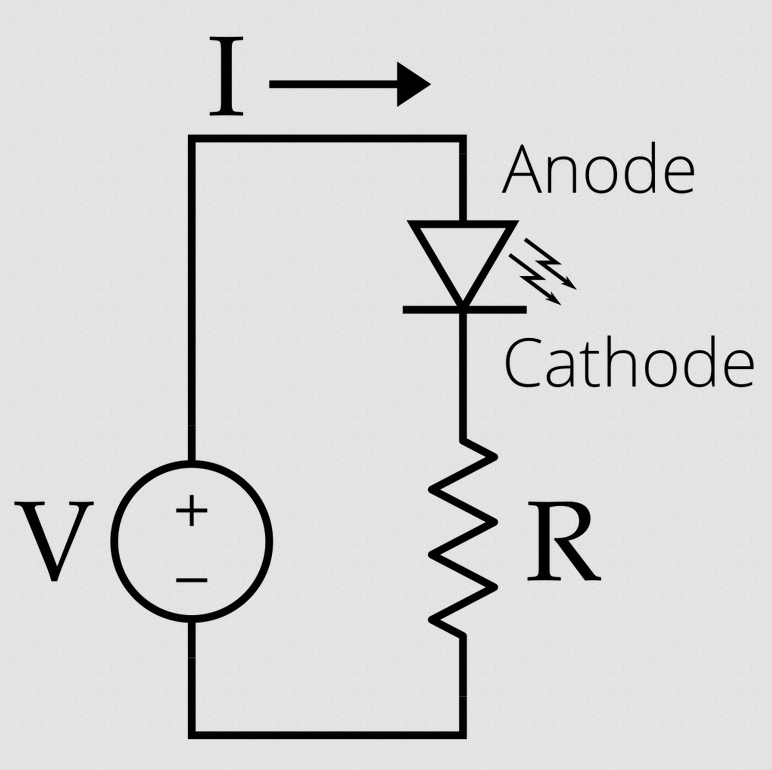
\includegraphics[width=8cm]{LED-Circuit.png}
    \caption{مدار دیود نوری}
    \label{fig:led-circ}
\end{figure}
\newline
\textcolor{red}{\begin{nas}سوال: \end{nas}}
با فرض اینکه ولتاژ دیود ۲ ولت باشد و منبع ولتاژ ۵ ولتی باشد، مقدار مقاومت سری را به گونه‌ای بیابید که جریان مدار ۱۵ میلی‌آمپر شود.
\newline
توجه کنید که دیود های نوری دو پایه دارند و پایه‌ای که بلند تر است پایانه‌ی مثبت دیود (آنود) و پایه‌ای که کوتاه تر است پایانه‌ی منفی (کاتود) دیود است. به هیچ عنوان دیود های نوری را به صورت برعکس در مدار قرار ندهید.
\pagebreak
\newline
\begin{nas}اتصال صحیح کلید به بورد\end{nas}
\newline
مدار زیر را در نظر بگیرید.
\newline
\begin{figure}[h]
    \centering
    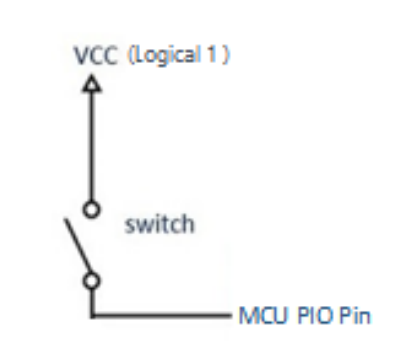
\includegraphics[width=8cm]{Switch-Direct.png}
    \caption{اتصال مستقیم کلید}
    \label{fig:swtch-dir}
\end{figure}
\newline
\textcolor{red}{\begin{nas}سوال: \end{nas}}
اگر کلید باز باشد ولتاژ \lr{MCU PIO Pin} چیست؟ این اتفاق چه مشکلی را پیش می‌آورد؟
\newline
برای حل مشکل مدار قبلی، باید از مقاومت های \lr{Pull Up} و \lr{Pull Down} استفاده کنیم. همانطور که از اسامی آنها پیداست، این مقاومت ها در هنگام قطع بودن کلید، ولتاژ را به بالا و یا به پایین می‌کشند. مدار های زیر را در نظر بگیرید:
\newline
\begin{figure}[h]
    \centering
    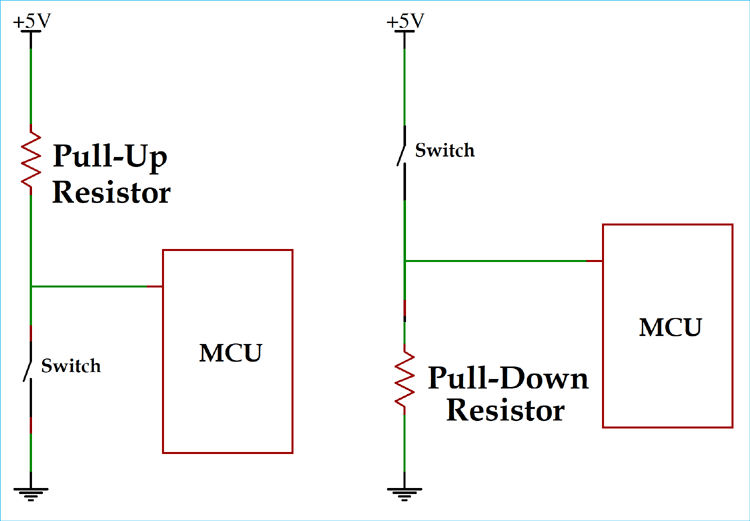
\includegraphics[width=8cm]{PUP-PDOWN.png}
    \caption{اتصال کلید با مقاومت های \lr{Pull Up} و \lr{Pull Down}}
    \label{fig:swtch-dir}
\end{figure}
\newline
\textcolor{red}{\begin{nas}سوال: \end{nas}}
ولتاژ ورودی به میکروکنترلر را در هر یک از مدار های بالا در حالت بسته و یا باز بودن میکروکنترلر محاسبه کنید.
\newline
\textcolor{red}{\begin{nas}سوال: \end{nas}}
بهتر است مقدار مقاومت استفاده شده مقدار بالایی باشد. دلیل این کار چیست؟
\newline
در نتیجه همواره برای اتصال یک کلید به میکروکنترلر از یکی از روش های \lr{Pull Up} و یا \lr{Pull Down} استفاده می‌کنیم.
\newline



\begin{nas}ورودی و خروجی\end{nas}
\newline
استفاده از پین های ورودی و خروجی از محیط آردوینو بسیار ساده‌است و با صدا زدن چند تابع انجام می‌شود.
\newline
\textcolor{red}{\begin{nas}سوال: \end{nas}}
در مورد توابع زیر تحقیق کنید و ورودی و خروجی هر تابع و کاری که انجام می‌دهند را بنوسید.
\begin{itemize}
    \item \lr{pinMode}
    \item \lr{digitalRead}
    \item \lr{digitalWrite}
    \item \lr{delay}
\end{itemize}




\begin{nas}وقفه\end{nas}
\newline
با وقفه ها در کلاس درس آشنا شدید. در سطوح پایین تر و نزدیک به سخت‌افزار به دلیل متفاوت بودن میکروکنترلر مورد استفاده در آزمایشگاه و میکروکنترلری که در کلاس درس تدریس شد، استفاده از وقفه ها مقداری متفاوت است اما به صورت کلی فرایند همان است.
\newline
\textcolor{red}{\begin{nas}سوال: \end{nas}}
انواع رویداد های ورودی که میکروکنترلر موجود در بورد \lr{Arduino Uno} می‌تواند تشخیص دهد و اعلام وقفه کند بنویسید.
\newline
\textcolor{red}{\begin{nas}سوال: \end{nas}}
کدام یک از پین های بورد شما قابلیت تشخیص وقفه را دارند؟
\newline
در محیط آردوینو استفاده از وقفه های مربوط به پین ورودی با استفاده از تابع \lr{attachInterrupt} صورت می‌گیرد.
\newline
\textcolor{red}{\begin{nas}سوال: \end{nas}}
در مورد تابع \lr{attachInterrupt} تحقیق کنید و ورودی و خروجی تابع و کاری که انجام می‌دهد را بنویسید.

\subsection{شرح آزمایش}

می‌خواهیم با استفاده از دیود نوری و کلید، یک شمارنده‌ی ۴ بیتی بسازیم. برای این کار، یک کلید را به همراه مقاومت \lr{Pull Up} یا \lr{Pull Down} به بورد متصل کنید و ۴ دیود نوری را نیز به هر یک از پین های بورد وصل کنید. فراموش نکنید که مقاومت سری ۲۲۰ اهمی را در مدار دیود های نوری قرار دهید.
سپس برنامه‌ای بنویسید که با استفاده از این ۴ دیود نوری از ۰ تا ۱۵ به صورت باینری شمارش کند و با هر بار فشردن کلید، یکی به عدد نمایش داده شده اضافه شود. برنامه را ابتدا به روش سرکشی و سپس به روش وقفه‌محور بنویسید.
\begin{itemize}
    \item به نظر شما اگر برنامه‌ی ما می‌خواست چند کار دیگر را نیز انجام دهد و شمردن با دیود نوری فقط یکی از وظایف آن بود، بهتر بود از کدام روش استفاده می‌کردیم؟
    \item اگر دکمه را برای مدت طولانی نگه دارید چه اتفاقی می‌افتد؟ دلیل این اتفاق چیست؟ برای حل این مشکل چه راه حلی دارید؟
\end{itemize}

\begin{figure}[h]
    \centering
    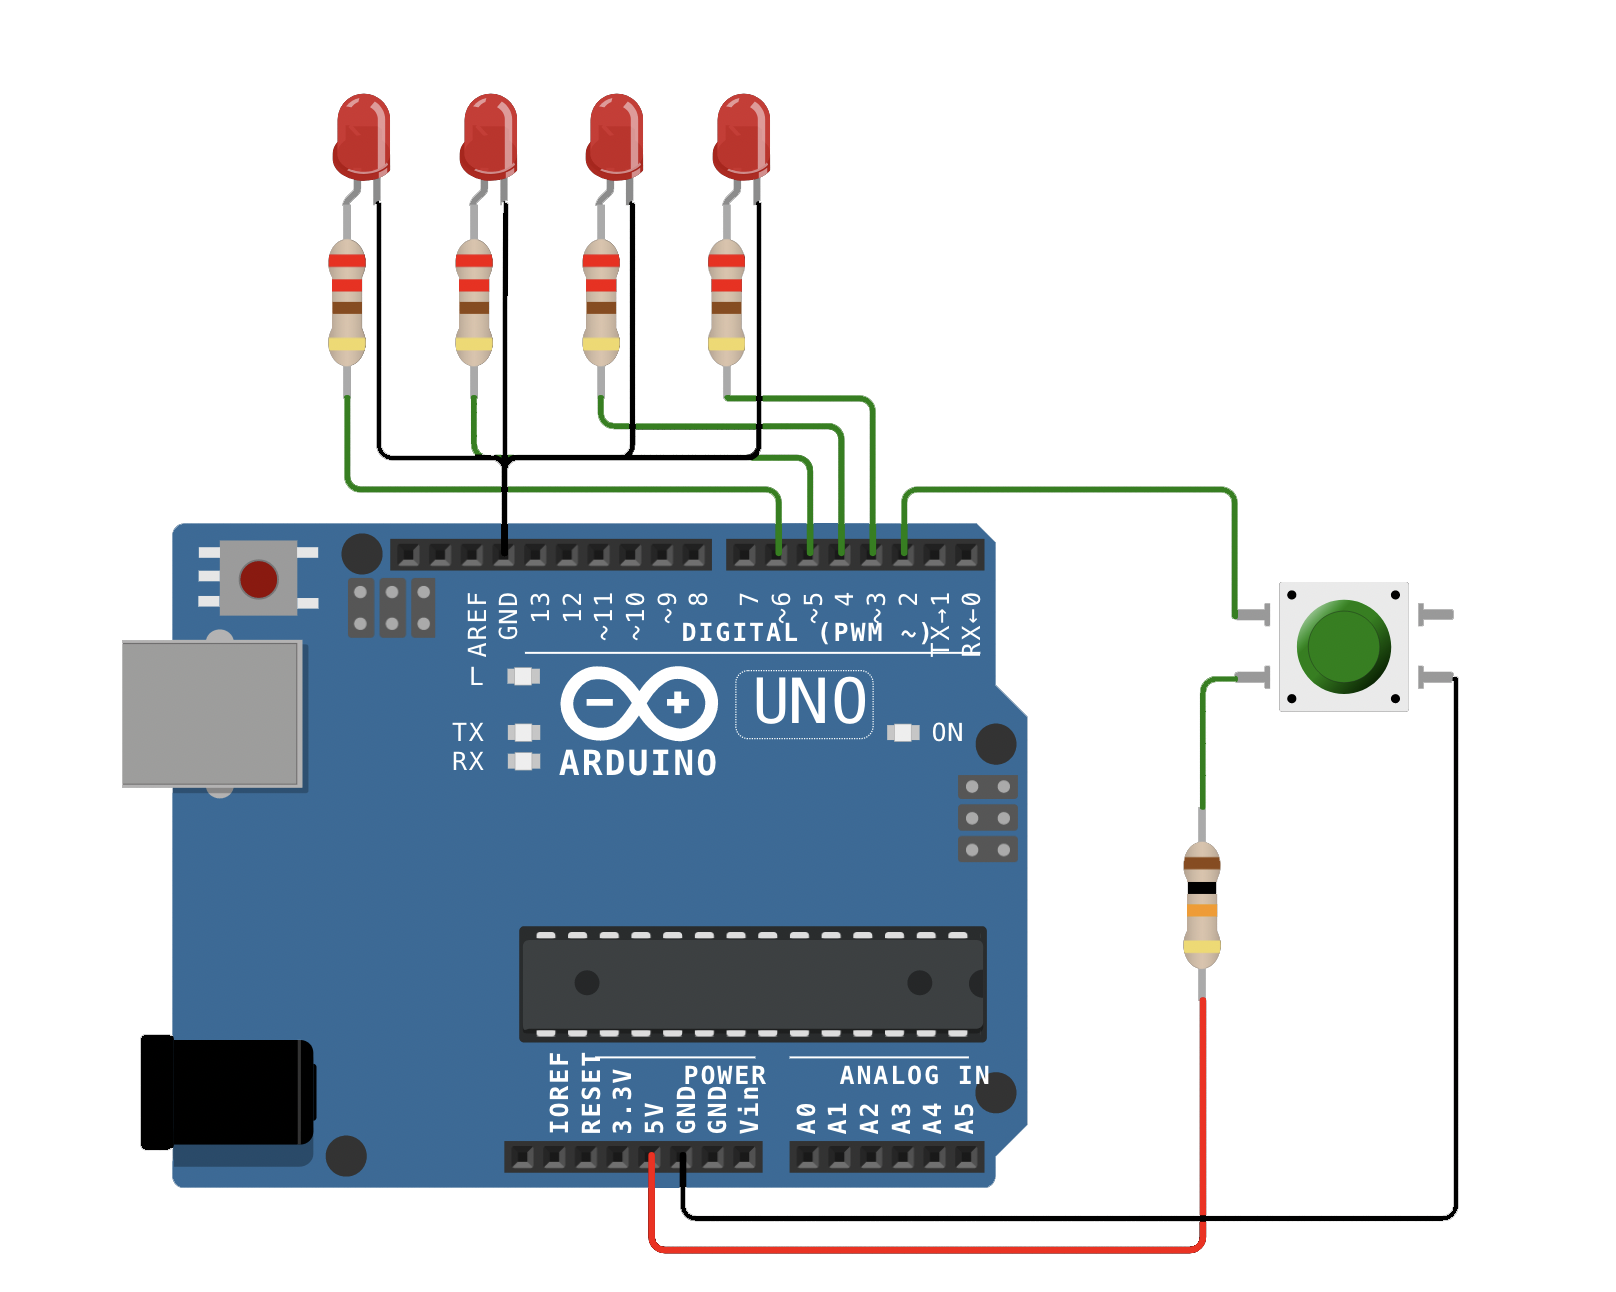
\includegraphics[width=16cm]{L1-Circuit.png}
    \caption{مدار آزمایش اول}
    \label{fig:l1circ}
\end{figure}

\pagebreak



\section{صفحه نمایش \lr{LCD} و صفحه کلید ماتریسی}

\subsection{اهداف آزمایش}
\begin{itemize}
    \item آشنایی با صفحه نمایش \lr{LCD} و صفحه کلید ماتریسی به عنوان رابط های کاربری
    \item آشنایی با نحوه‌ی اضافه کردن کتاب‌خانه ها در محیط آردوینو
\end{itemize}

\subsection{قطعات مورد نیاز}
\begin{itemize}
    \item \lr{Arduino Uno}
    \item صفحه نمایش \lr{LCD}
    \item صفحه کلید ماتریسی
    \item پتانسیومتر ۱ کیلواهم \lr{B1K}
    \item مقاومت ۲۲۰ اهم
\end{itemize}
\pagebreak

\subsection{مقدمه}

\begin{nas}یاد آوری مقسم ولتاژ و پتانسیومتر\end{nas}
\newline
در درس و آزمایشگاه مدار های الکتریکی با مدار مقسم ولتاژ آشنا شدید. این مدار در واقع از ۲ مقاومت سری تشکیل شده که ولتاژ ورودی میان آنها تقسیم می‌شود.
\newline
\begin{figure}[h]
    \centering
    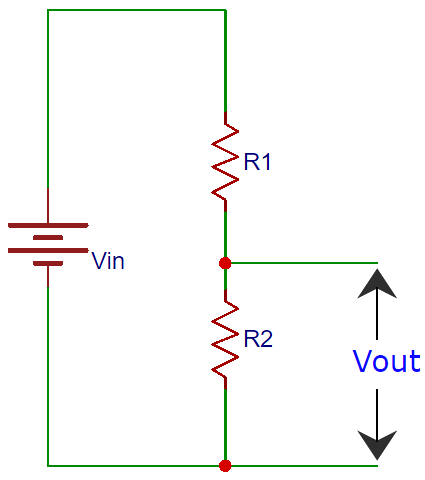
\includegraphics[width=4cm]{vdiv.png}
    \caption{مدار مقسم ولتاژ}
    \label{fig:voldiv}
\end{figure}
\newline
با استفاده از \lr{KVL} به سادگی به فرمول زیر می‌رسیم:
\begin{equation}V_{out} = V_{in} \times \frac{R2}{R1 + R2}\end{equation}
استفاده‌ی اصلی ما از این مدار، کم کردن ولتاژ ورودی به یک وسیله‌است. پتانسیومتر ها مقسم های ولتاژی هستند که مقدار مقاومت های \lr{R1} و \lr{R2}در آنها (معمولا با چرخاندن سر پتانسیومتر) قابل تغییر است و در این آزمایش برای کنترل کنتراست صفحه نمایش از آن استفاده می‌کنیم.
\newline
\begin{figure}[h]
    \centering
    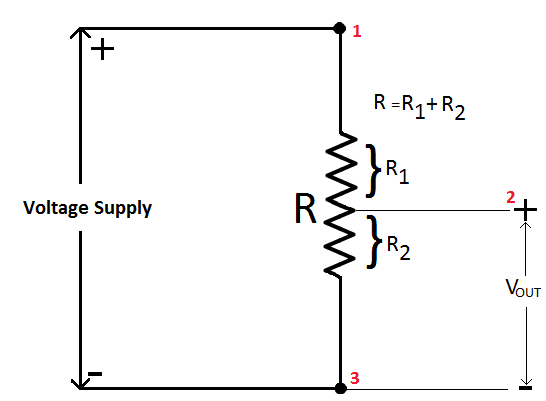
\includegraphics[width=8cm]{pot.png}
    \caption{مدار معادل یک پتانسیومتر. توجه کنید هنگامی که می‌گوئیم یک پتانسیومتر ۱۰ کیلو اهمی، ۱۰ کیلو اهم بیانگر مقدار \lr{R} است.}
    \label{fig:pot-circ}
\end{figure}
\newline
\begin{nas}صفحه نمایش \lr{LCD}\end{nas}
\newline
صفحه نمایش کاراکتری \lr{16x2} یکی از روش های متداول ارتباط با کاربر در سیستم های نهفته‌است. منظور از \lr{16x2} اندازه‌ی صفحه نمایش است، یعنی این صفحه های نمایش قابلیت نشان دادن ۲ ردیف و ۱۶ ستون از کاراکتر ها را دارند. خود صفحه نمایش توسط یک \lr{IC} کنترل می‌شود که میکروکنترلر ما باید با آن ارتباط برقرار کند. ابتدا با پین های ورودی یک ماژول صفحه‌نمایش کاراکتری آشنا می‌شویم:
\newline
\begin{figure}[h]
    \centering
    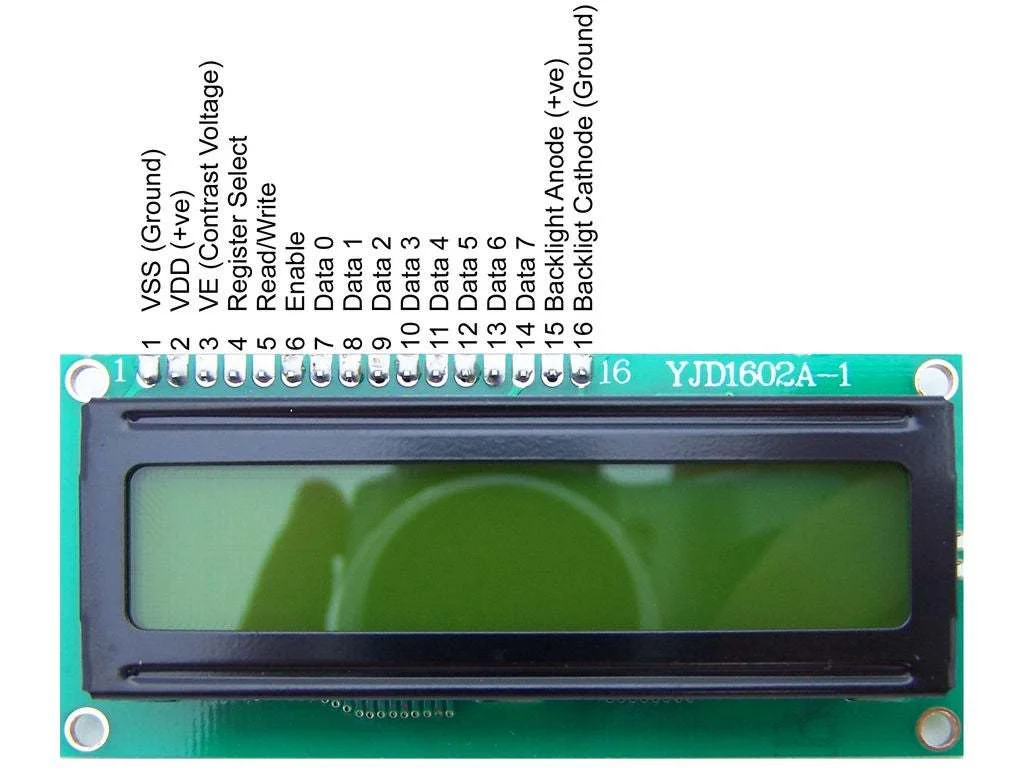
\includegraphics[width=8cm]{lcd_pinout.png}
    \caption{نمایی از یک صفحه نمایش کاراکتری ۱۶ در ۲}
    \label{fig:lcd-pinout}
\end{figure}
\begin{itemize}
    \item پین شماره ۱: ولتاژ \lr{Ground}
    \item پین شماره ۲: ولتاز \lr{Vcc}
    \item پین شماره ۳: کنترل کنتراست. با استفاده از یک پتانسیومتر می‌توانیم کنتراست صفحه نمایش را کنترل کنیم
    \item پین های شماره ۴ تا ۶: پین های کنترلی
    \item پین های شماره ۷ تا ۱۴:‌پین های ورودی داده
    \item پین های شماره ۱۵ و ۱۶: به ترتیب آنود و کاتود \lr{Backlight LED}. توجه کنید این پین ها مستقیما به یک \lr{LED} متصل می‌شوند و ارتباطی با آی‌سی کنترلر ندارند. طبیعتا مانند دیگر \lr{LED} ها حتما برای جلوگیری از خرابی قطعه باید یک مقاومت با آن سری قرار دهید.
\end{itemize}
\pagebreak
از آنجایی که ما از کتاب‌خانه های مخصوص ارتباط با \lr{LCD} استفاده خواهیم کرد، نیازی به دانستن جزئیات این ارتباط نیست و در صورت علاقه می‌توانید خودتان از دیتاشیت مربوطه مطالعه کنید، اما باید نحوه‌ی کار با کتابخانه را بلد باشید و بتوانید از آن استفاده کنید.
\newline
\textcolor{red}{\begin{nas}سوال: \end{nas}}
\newline
در مورد توابع زیر از کتابخانه‌ی \lr{LiquidCrystal.h} تحقیق کنید و ورودی و خروجی توابع و کاری که انجام می‌دهند را بنویسید.
\begin{itemize}
    \item \lr{LiquidCrystal()}
    \item \lr{begin()}
    \item \lr{clear()}
    \item \lr{home()}
    \item \lr{setCursor()}
    \item \lr{write()}
    \item \lr{print()}
\end{itemize}

\pagebreak
\begin{nas}صفحه کلید ماتریسی\end{nas}
\newline
در آزمایش قبلی از کلید های معمولی برای گرفتن ورودی از کاربر استفاده کردیم. اگر بخواهیم مانند روش آزمایش قبل ۱۶ عدد کلید برای ورودی داشته باشیم به مشکل می‌خوریم، چون تعداد پین های ورودی میکروکنترلر ما محدود است. به همین دلیل باید از روش ماتریسی برای اتصال کلید ها به میکروکنترلر استفاده کنیم.
\newline
در این روش کلید ها به صورت زیر در یک جدول قرار می‌گیرند:
\newline
\begin{figure}[h]
    \centering
    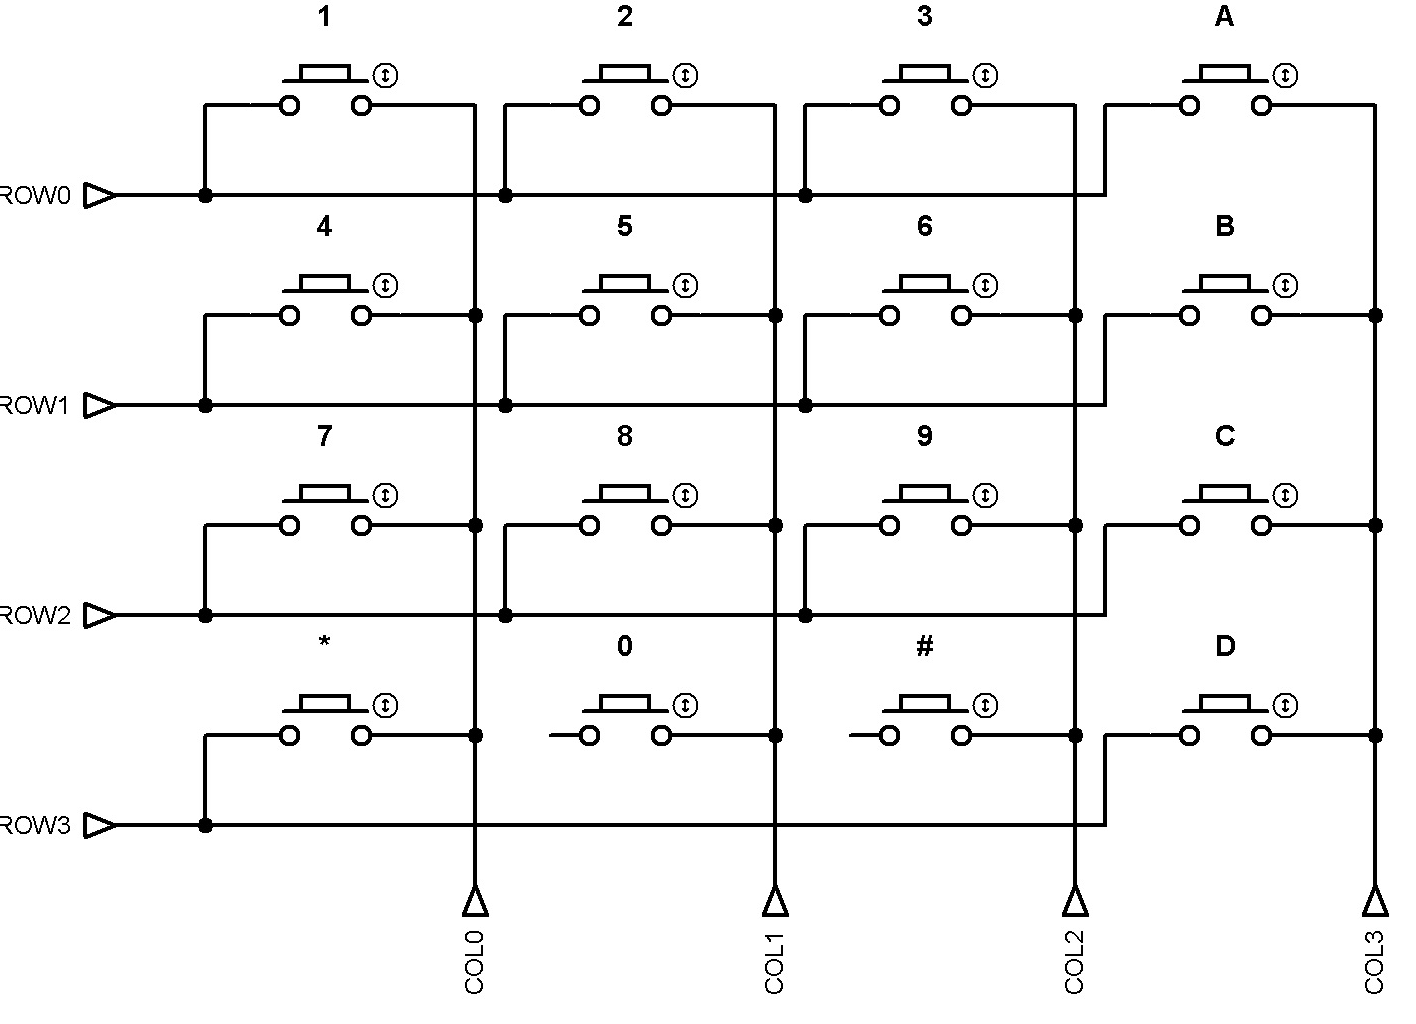
\includegraphics[width=16cm]{keypad-circ.png}
    \caption{مدار یک صفحه کلید ماتریسی}
    \label{fig:keypad-circ}
\end{figure}
\newline
برای استفاده از این مدار، باید به همه‌ی سطر ها ولتاژ صفر منطقی بدهیم و ستون ها را با استفاده از
\lr{Pull Up Resistor} به ورودی های میکروکنترلر وصل کنیم.
هنگامی که یک کلید بسته می‌شود سطر و ستون متناظر با آن متصل می‌شوند و ورودی آن ستون به میکروکنترلر از یک به صفر منطقی تغییر پیدا می‌کند. در این مرحله می‌دانیم که یک کلید در ستونی که ورودیش تغییر کرده روشن شده است. برای اینکه سطر آن را نیز پیدا کنیم و بفهمیم کدام کلید روشن شده، یک به یک سطر ها را به یک منطقی تغییر می‌دهیم. اگر هنگامی که یک سطر به یک منطقی تغییر کرد، ستون نیز به یک منطقی تغییر کند سطری که کلید در آن قرار دارد را نیز پیدا کرده‌ایم و تشخیص دادیم که کدام کلید بسته شده بود.

\newline
\textcolor{red}{\begin{nas}سوال: \end{nas}}
شبه کد/فلوچارت استفاده از صفحه کلید ماتریسی را بنویسید.
\newline

برای کار با صفحه کلید نیز از کتاب‌خانه های مخصوص به آن استفاده می‌کنیم که نام آن \lr{Keypad.h} است.
برای دریافت این کتاب‌خانه، از منوی سمت راست \lr{Arduino IDE} به قسمت \lr{Library Manager} بروید و کتابخانه‌ی \lr{Keypad by Mark Stanley} را دریافت نمایید. مستندات مربوط به این کتاب‌خانه را می‌توانید در 
\href{https://playground.arduino.cc/Code/Keypad/}{این لینک}
مشاهده کنید.
\newline
\textcolor{red}{\begin{nas}سوال: \end{nas}}
در مورد توابع زیر از کتابخانه‌ی \lr{Keypad.h} تحقیق کنید و ورودی و خروجی توابع و کاری که انجام می‌دهند را بنویسید.
\begin{itemize}
    \item \lr{Keypad()}
    \item \lr{begin()}
    \item \lr{waitForKey()}
    \item \lr{getKey()}
\end{itemize}
\newline
\subsection{شرح آزمایش}

می‌خواهیم یک ماشین‌حساب درست کنیم. ابتدا مانند مداری که در انتهای آزمایش در اختیار شما قرار گرفته، صفحه نمایش و صفحه کلید را به آردوینو متصل کنید. نیازی نیست مدار شما دقیقا همان مدار باشد، اما توجه کنید که به هیچ عنوان قرار دادن مقاومت و پتانسیومتر در مدار را فراموش نکنید. در صورتی که پتانسیومتر ندارید، می‌توانید به پین \lr{Vo} یک مقاومت ۳.۳ کیلواهمی متصل به زمین وصل کنید. همچنین وقتی صفحه کلید ماتریسی رو به روی شما باشد و پین‌ها رو به پایین باشند، پین‌ها از چپ به راست ابتدا پین های ردیف‌ها هستند و سپس پین های ستون‌ها هستند. برنامه‌ای بنویسید که کلید ها را از صفحه کلید بخواند و آنها را روی صفحه‌نمایش نمایش دهد و بعد از اینکه کلید \lr{=} زده شد، عبارت ریاضی که کاربر وارد کرده را محاسبه کرده و مقدار آن را روی صفحه‌نمایش نمایش دهد.
توجه کنید نیازی به رعایت اولویت ها و پشتیبانی از اعداد اعشاری و اعداد منفی نیست.

\begin{figure}[h]
    \centering
    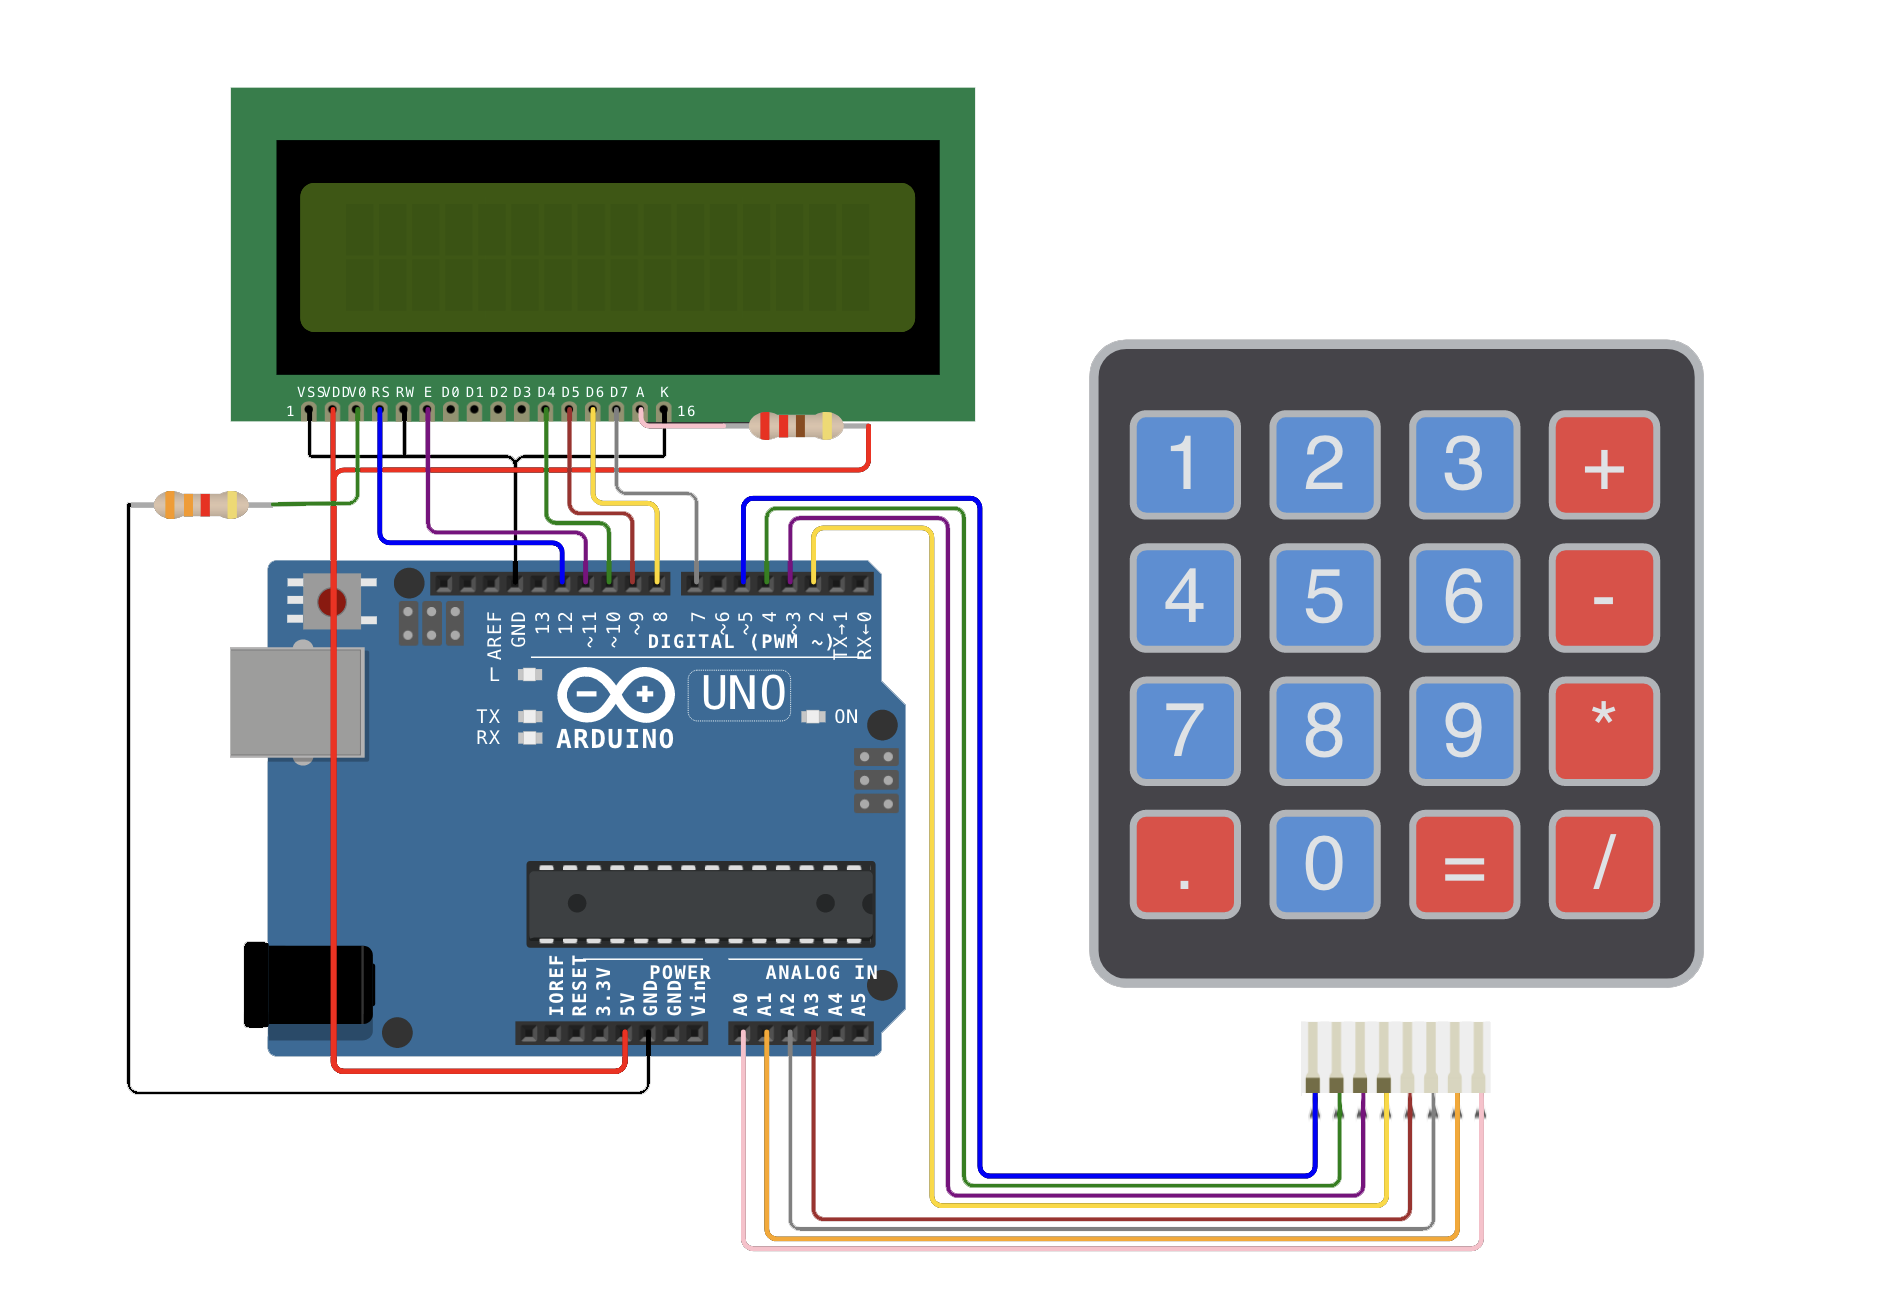
\includegraphics[width=14cm]{L2-Circuit.png}
    \caption{مدار مربوط به آزمایش دوم}
    \label{fig:l2-circ}
\end{figure}

\newline
\section{صفحه نمایش ماتریسی}

\subsection{اهداف آزمایش}
\begin{itemize}
    \item آشنایی با پروتوکل \lr{SPI}
    \item آشنایی با صفحه نمایش ماتریسی
\end{itemize}
\subsection{قطعات مورد نیاز}

\begin{itemize}
    \item بورد \lr{Arduino Uno}
    \item صفحه نمایش ماتریسی به همراه چیپ \lr{MAX7219}
\end{itemize}
\subsection{مقدمه}

در این آزمایش می‌خواهیم با با استفاده از یک صفحه نمایش ماتریسی، یک متن را به سبک تابلوهای روان تبلیغاتی نمایش دهیم. ابتدا باید با مفاهیم پایه‌ای مربوط به صفحه‌نمایش ماتریسی و چیپ \lr{MAX7219} آشنا شویم.

\newline
\begin{nas} صفحه نمایش ماتریسی\end{nas}
\newline

به طور عادی برای کنترل یک صفحه نمایش ماتریسی ۸ در ۸، به ۶۴ پین کنترلی نیاز داریم. این کار نه با میکروکنترلر مورد استفاده ما قابل انجام است، و نه مقیاس پذیری خوبی دارد و مشخصا صفحه نمایش‌های امروزی که میلیون ها پیکسل دارند نیاز به میلیون‌ها پین کنترلی ندارند. برای حل این مشکل از تکنیکی به نام مالتی‌پلکسینگ استفاده می‌شود. در این روش دیودهای نوری در ۸ ردیف و ۸ ستون قرار می‌گیرند.
\newline
\textcolor{red}{\begin{nas}سوال: \end{nas}}
در مورد روش مالتی‌پلکسینگ تحقیق کنید و مختصرا توضیح دهید. چگونه با این روش یک تصویر کامل به نمایش در می‌آید؟

\newline
\begin{nas}چیپ \lr{MAX7219}\end{nas}
\newline

چیپ \lr{MAX7219}
برای ما کار مالتی‌پلکسینگ و کنترل صفحه‌نمایش را انجام می‌دهد. نحوه ارتباط با این ماژول با استفاده از پروتوکل ارتباطی \lr{SPI} است. در این ارتباط باید دستورات مشخصی را برای چیپ بفرستیم و چیپ با توجه به دستورات ارسالی ما صفحه‌نمایش را کنترل می‌کند. در واقع این چیپ شامل تعدادی رجیستر کنترلی است که ما باید مقادیر آن را کنترل کنیم. برای کنترل هر کدام از این رجیسترها ابتدا در یک باید آدرس رجیستر فرستاده می‌شود و سپس در یک بایت دیگر مقدار ارسالی فرستاده می‌شود.

\newline
\textcolor{red}{\begin{nas}سوال: \end{nas}}
در ابتدای کار با این چیپ، باید تعداد \lr{Scan Line} ها برابر هشت قرار داده شود. در دیتاشیت این چیپ بگردید و آدرس رجیستر مربوطه، مقداری که باید به آن داده شود و همچنین قطعه کد آردوینو مربوط به تعیین این رجیستر را بنویسید.

\newline
\textcolor{red}{\begin{nas}سوال: \end{nas}}
در ابتدای کار با این چیپ، باید  
\lr{Test Mode}
غیر فعال شود. در دیتاشیت این چیپ بگردید و آدرس رجیستر مربوطه، مقداری که باید به آن داده شود و همچنین قطعه کد آردوینو مربوط به تعیین این رجیستر را بنویسید

\newline
\textcolor{red}{\begin{nas}سوال: \end{nas}}
روشن و خاموش بودن ال‌ای‌دی ها به صورت ردیفی کنترل می‌شود. برای کنترل هر ردیف ابتدا یک بایت ردیف مورد نظر و سپس یک بایت ال‌ای‌دی های روشن به صورت کدینگ باینری فرستاده می‌شود. در این کدینگ هر بیت یک معادل یک ال‌ای‌دی روشن در ردیف مورد نظر است. قطعه کد آردوینو مربوط به روشن کردن ال‌ای‌دی پنجم ردیف چهارم را بنویسید.

\subsection{شرح آزمایش}

\begin{enumerate}
    \item ماژول صفحه‌نمایش را به آردوینو متصل کنید. پین‌های \lr{VCC} و \lr{GND} به ترتیب به ۵ ولت و زمین وصل می‌شوند و پین‌های دیگر که مربوط به ارتباط \lr{SPI} هستند را می‌توانید از قسمت راهنمای پین‌های آردوینو در دستور کار مشاهده کنید. توجه کنید که به دلیل اینکه صفحه‌نمایش داده‌ای ارسال نمی‌کند پین \lr{MISO} نداریم و پین \lr{MOSI} نیز روی ماژول ممکن است به اسم \lr{DIN} نوشته شده باشد. پین چیپ سلکت را به یکی از پین های دیجیتال متصل کنید.
    \item کدی بنویسید که عبارت \lr{HELLO} را به صورتی که هر ثانیه یکی از کاراکترهای عبارت روی صفحه‌نمایش باشند نمایش دهد.
\end{enumerate}
\section{کتابخوان}

\subsection{اهداف آزمایش}
\begin{itemize}
    \item آشنایی با پروتکل ارتباط سریال \lr{I2C}
    \item کار با حافظه‌ی \lr{EEPROM} بیرونی و نحوه‌ی خواندن از آن
\end{itemize}
\subsection{قطعات مورد نیاز}
\begin{itemize}
    \item \lr{Arduino Uno}
    \item صفحه نمایش \lr{LCD}
    \item پتانسیومتر ۱ کیلواهم \lr{B1K}
    \item مقاومت ۲۲۰ اهم
    \item \lr{EEPROM (AT24C16)}
    \item کلید \lr{Switch}
    \item مقاومت ۱۰ هزار اهم
\end{itemize}
\subsection{مقدمه}
در این آزمایش میخواهیم با نحوه کار با حافظه 
\lr{EEPROM}
آشنا شویم و از آن برای نمایش دادن یک کتاب که متن آن درون این حافظه‌ی بیرونی ذخیره شده استفاده کنیم. برای نمایش دادن خط به خط کتاب بر روی
\lr{LCD}
با استفاده از ۲ کلیدی که در مدار قرار می‌دهیم به خط قبلی یا خط بعدی کتاب می‌رویم.

\newline
\begin{nas}حافظه \lr{EEPROM}\end{nas}
\newline

در بسیاری از برنامه ها ما نیاز داریم که اطلاعاتی را ذخیره کنیم تا پس از اجرای مجدد برنامه از آنها استفاده کنیم. همچنین اطلاعاتی که حجم زیادی دارند را نمی‌توان در حافظه‌ی خود برد ذخیره کرد و نیاز داریم که یک حافظه بیرونی برای ذخیره این اطلاعات داشته باشیم که پس از متوقف کردن برنامه نیز اطلاعات در آن ذخیره بمانند. همچنین در دنیای میکروکنترلر ها یکی از اصلی ترین مسائلی که قیمت میکروکنترلر های مختلف را متفاوت می‌کند میزان حافظه‌ی آنهاست و یکی از راه هایی که می‌توان قیمت تمام شده‌ی یک محصول دارای یک سیستم نهفته را کمتر کرد استفاده از میکروکنترلری با حافظه‌ی کمتر و وصل کردن یک حافظه‌ی بیرونی به آن است.
 به همین دلیل ما به \lr{EEPROM} ها نیاز داریم.
\newline
در یک دسته‌بندی می‌توان \lr{EEPROM} ها را به دو نوع درونی و بیرونی دسته‌بندی کرد. حافظه‌های درونی در کنار پردازنده بر روی همان مدار مجتمع قرار می‌گیرند و نیازی به استفاده از پایه های آدرس ندارند. همچنین به دلیل حضور در یک مدار مجتمع اتصال بهتری میان آن‌ها و میکروکنترلر برقرار است و سرعت آن‌ها بیشتر است. بورد \lr{Arduino Uno} نیز یک حافظه ی \lr{EEPROM} درونی به اندازه ۱ کیلوبایت دارد که در این آزمایش مورد توجه ما نیست.
\newline
 گونه‌ای دیگر از 
 \lr{EEPROM}
 ها بیرونی هستند که بر روی یک 
 \lr{IC}
 جداگانه قرار میگیرند. برای ارتباط با این حافظه‌ها اکثرا از پروتکل‌های ارتباط سریال استفاده میشود. حافظه 
 \lr{AT24C16}
 نیز که در این آزمایش به کار برده میشود، پروتکل سریال 
 \lr{TWI}
 را به کار میگیرد. به این صورت که در این پروتکل حافظه‌ها همان برده‌ها 
 \lr{(Slaves)}
 هستند و برد کنترلر نیز سرپرست  
 \lr{(Master)}
 است. در این دسته گاهی برای اینکه بتوان چند حافظه را بر روی یک باس کنترل کرد (چند برده داشت) از پایه‌های آدرس استفاده میشود. این آدرس به صورت سخت‌افزاری پیکربندی میشود 
 \lr{(Hard-Wired)}
 .
\newline

\lr{AT24C16}
از پروتکل 
\lr{TWI}
یا همان \lr{I2C} استفاده می‌کند و مطابق چیزی که از این پروتکل می‌دانیم باید ۷ بیت آدرس داشته باشد. چهار بیت پر ارزش آدرس آن مقدار ثابت \lr{0b1010} است و سه بیت کم ارزش آن را پایه های
\lr{A0} تا \lr{A3}
مشخص می‌کند. البته این پایه ها در واقعیت ممکن است استفاده بشوند یا نشوند. در واقع چیپ حافظه‌ی \lr{AT24C16} از این پین ها استفاده نمی‌کند و همواره سه بیت کم ارزش آدرس آن صفر است و چیپ \lr{AT24C08} نیز فقط از پین \lr{A2} استفاده می‌کند و دو پین دیگر همواره صفر هستند. همیشه برای اینگونه فهمیدن جزئیات کار با قطعات الکترونیکی به دیتاشیت قطعه مراجعه کنید.
\newline
همچنین 
\lr{EEPROM}
پایه ای به نام 
\lr{WP}
دارد که مخفف 
\lr{Write Protection}
است که اگر مقدار منطقی آن برابر یک باشد و به عبارتی به آن ولتاژ وارد شود، فعال میشود و امکان نوشتن روی 
\lr{EEPROM}
دیگر وجود ندارد.
دو تصویر از پایه های 
\lr{AT24C16}
و کارکرد هرکدام از آن‌ها نمایش داده شده است.

\newline
\begin{figure}[h]
    \centering
    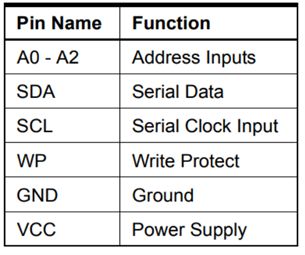
\includegraphics[width=8cm]{eeprom-pindesc.png}
    \caption{کارکرد پین های حافظه}
    \label{fig:eeprom-pindesc}
\end{figure}

\begin{figure}[h]
    \centering
    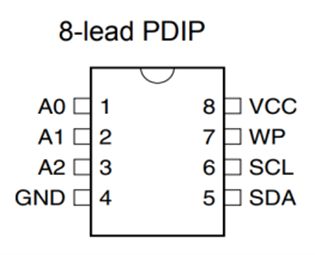
\includegraphics[width=8cm]{eeprom-pinout.png}
    \caption{دیاگرام پین های حافظه}
    \label{fig:eeprom-pinout}
\end{figure}
\newline

\begin{nas} کار با کتابخانه \lr{TWI} در \lr{Arduino} \end{nas}
\newline

کتابخانه 
\lr{wire.h}
یکی از کتابخانه‌های استاندارد آردوینو است که نیازی به نصب آن نیست. این کتابخانه توابع لازم برای کار با پروتکل \lr{TWI} را فراهم میکند. برخی از توابع این کتابخانه به شرح زیر است:
\begin{itemize}
    \item \lr{begin()}
    \item \lr{setClock()}
    \item \lr{beginTransmission()}
    \item \lr{write()}
    \item \lr{endTransmission()}
    \item \lr{requestFrom()}
    \item \lr{available()}
    \item \lr{read()}
\end{itemize}

\textcolor{red}{\begin{nas}سوال: \end{nas}}
هر یک از توابع بالا را در مستندات کتابخانه بررسی کنید و ورودی ها، خروجی ها و عملکرد آنها را توضیح دهید.
\pagebreak
\newline

\begin{nas}چگونگی خواندن و نوشتن بر روی حافظه‌ی \lr{EEPROM}\end{nas}
\newline
الگوریتم خواندن به صورت زیر است:
\begin{enumerate}
    \item شروع ارتباط با دستگاهی که آدرس \lr{I2C} آن آدرس حافظه‌ی ما است.
    \item نوشتن یک بایت آدرس حافظه‌ای که می‌خواهیم بخوانیم.
    \item پایان ارتباط.
    \item درخواست تعداد بایت دلخواه از دستگاهی که آدرس \lr{I2C} آن آدرس حافظه‌ی ما است.
    \item به اندازه‌ی بایت هایی که درخواست کردیم داده می‌خوانیم.
\end{enumerate}

الگوریتم نوشتن به صورت زیر است:
\begin{enumerate}
    \item شروع ارتباط با دستگاهی که آدرس \lr{I2C} آن آدرس حافظه‌ی ما است.
    \item نوشتن یک بایت آدرس حافظه‌ای که می‌خواهیم در آن بنویسیم.
    \item نوشتن بایت هایی که می‌خواهیم بنویسیم.
    \item پایان ارتباط.
\end{enumerate}

\subsection{شرح آزمایش}

\paragraph{
ابتدا اتصالات مربوط به حافظه را کامل کنید. مشخصا پایه های \lr{VCC} و \lr{GND} باید به مثبت و زمین وصل شوند. همه پایه های آدرس و پایه \lr{WP} را نیز به زمین وصل کنید. پایه های کلاک و دیتا را باید به پایه های مخصوص کلاک و دیتای پروتکل \lr{I2C} آردوینو وصل کنید. نقشه‌ای از پین های آردوینو در قسمت «راهنمای پین‌های آردوینو» آمده که می‌توانید از آن استفاده کنید.
}

\paragraph{
یک چیپ حافظه به شما داده می‌شود که از قبل روی آن یک متن ذخیره شده. شما باید ۱۶ کاراکتر از این متن را بخوانید و روی صفحه‌نمایش نمایش دهید. همچنین دو کلید داشته باشید که با فشردن این دو کلید دستگاه شما ۱۶ کاراکتر بعدی یا قبلی متن را بخواند و نمایش دهد. 
توجه کنید نیازی به نوشتن چیزی بر روی حافظه نیست و این کار از قبل برای شما انجام شده است.
}
\section{کار با سنسور \lr{LM35} و استفاده از آن در ساخت فن هوشمند بر اساس دما}

\subsection{اهداف آزمایش}
\begin{itemize}
    \item آشنایی با سنسور دمای \lr{LM35}
    \item آشنایی با نحوه‌ی کار با ترانزیستور برای سوییچینگ و استفاده از منبع تغذیه خارجی
\end{itemize}
\subsection{قطعات مورد نیاز}
\begin{itemize}
    \item بورد \lr{Arduino Uno}
    \item سنسور \lr{LM35}
    \item موتور \lr{DC}
    \item ترانزیستور \lr{BC140}
    \item دیود \lr{1N4001}
    \item منبع تغذیه
    \item مقاومت ۱ کیلواهم
\end{itemize}

\subsection{مقدمه}

\begin{nas} سنسور \lr{LM35} \end{nas}
\newline
\lr{LM35} یک سنسور دمای ولتاژ پایین به درجه سانتی‌گراد است. خروجی این سنسور یک ولتاژ است که به طور خطی با دما به درجه سانتی‌گراد متناسب است و کار با آن بسیار آسان است.
\newline
این سنسور نیازی به کالیبراسیون ندارد و دقت آن ۱ درجه سانتی‌گراد در محدوده دمایی -۵۵ تا +۱۵۵ است. این سنسور می‌تواند با منبع تغذیه ۴ تا ۳۰ ولت تغذیه شود و مصرف جریانی کمتر از ۶۰ میکروآمپر دارد.
\newline
\lr{LM35} در سه شکل مختلف عرضه می‌شود اما رایج ترین نوع آن بسته ۳ پین است که شکلی مشابه یک ترانزیستور دارد.

\newline
\textcolor{red}{\begin{nas}سوال: \end{nas}}
در رابطه با پایه های سنسور \lr{LM35} تحقیق کرده و وظیفه و محدوده ولتاژ ورودی و خروجی قابل قبول هر پایه را بنویسید. برای این کار می‌توانید به دیتاشیت این سنسور مراجعه کنید. محدودی های ولتاژی و جریانی معمولا در قسمتی از دیتاشیت به اسم \lr{Electrical Characteristics} قرار دارند.
\newline

پایه خروجی \lr{LM35} به یکی از ورودی های آنالوگ آردوینو متصل می‌شود. مقدار این ورودی را می‌تواند با تابع \lr{analogRead} خواند.
\newline
\textcolor{red}{\begin{nas}سوال: \end{nas}}
در رابطه با تابع \lr{analogRead} تحقیق کنید و در مورد ورودی و خروجی این تابع توضیح دهید. خروجی این تابع چیست و در چه محدوده‌ای قرار دارد؟
\newline

برای تبدیل خروجی تابع \lr{analogRead} به مقدار دمایی که سنسور به ما می‌دهد باید ابتدا این خروجی را به مقدار بین ۰ تا ۵ ولت تبدیل کرده و سپس آن را ضرب در ۱۰۰ کنید.
\newline
\textcolor{red}{\begin{nas}سوال: \end{nas}}
شبه کد تبدیل خروجی \lr{analogRead} به دما را بنویسید.

\newline
\begin{nas}ترانزیستور\end{nas}
\newline
آردوینو تنها می تواند ۴۰ میلی آمپر در ولتاژ ۵ ولت را روی پین های دیجیتال خود ارائه دهد. اکثر موتورها برای کار کردن به جریان ویا ولتاژ بیشتری نیاز دارند. یک ترانزیستور می تواند به عنوان یک سوئیچ دیجیتال عمل کند و آردوینو را قادر می سازد تا بارهای با نیازهای الکتریکی بالاتر را کنترل کند. به این صورت که ما از پین خروجی آردوینو صرفا برای خاموش و روشن کردن کلید استفاده می‌کنیم و جریان تغذیه اصلی را از یک منبع تغذیه خارجی می‌گیریم.
\newline
ترانزیستور ها دارای سه پایه هستند. در ترانزیستور های پیوندی دوقطبی یا \lr{Bipolar Junction Transistor} این پایه ها بیس، امیتر و کلکتور نام دارند. نحوه‌ی کار آنها به زبان ساده به این صورت است که عبور جریانی کوچک در پایه‌ بیس باعث این می‌شود که جریانی بسیار بزرگ‌تر از پایه کلکتور به امیتر برود. این ترانزیستور ها در دو نوع \lr{pnp} و \lr{npn} وجود دارند که اشاره به ساختار داخلی آن دارند.
\newline
توجه کنید که به دلیل ساختار داخلی ترانزیستور های دوقطبی جهت جریان عبوری بین پایه های امیتر و کلکتور مهم است. به اسم پایه ها توجه کنید، پایه امیتر همانطور که از اسمش پیداست وظیفه تزریق حامل بار و پایه کلکتور وظیفه‌ی جمع‌آوری آنها را دارد. در ترانزیستور های \lr{npn} حامل بار الکترون است پس جهت الکترون ها از امیتر به کلکتور و جهت جریان از کلکتور به امیتر است. در ترانزیستور های \lr{pnp} اما برعکس این است و جریان از امیتر به کلکتور است.
در قرار دادن ترانزیستور در مدار حتما به این نکته توجه کنید.
\newline
\textcolor{red}{\begin{nas}سوال: \end{nas}}
با توجه به نکته‌ای که گفته شد، در هر کدام از ترانزیستور های \lr{npn} و \lr{pnp} مشخص کنید که کدام یک از پایه های امیتر و کلکتور به موتور و منبع تغذیه متصل می‌شوند.

\newline
\begin{nas}موتور \lr{DC}\end{nas}
\newline
موتورهای \lr{DC} از طریق القای مغناطیسی کار می‌کنند. هنگامی که جریان وارد سیم یک میدان مغناطیسی ایجاد می‌شود. با افزایش جریان میدان مغناطیسی قوی‌تر شده و ارتباط این میدان مغناطیسی با آهن ربا های داخل موتور سبب چرخیده شدن شفت مرکزی موتور می‌شود. برعکس این عملیات نیز صادق است، یعنی با چرخاندن موتور می‌توانیم تولید جریان کنیم. به همین دلیل باید در مدار یک دیود نیز قرار دهیم تا در صورتی که موتور ما به هر دلیلی تولید جریان کرد از عبور این جریان جلوگیری شده تا باعث آسیب رساندن به قطعات نشود.

\subsection{شرح آزمایش}
\begin{enumerate}
    \item در هیچکدام از مراحل گفته شده قبل از دو مرحله آخر آردوینو متصل به برق و روشن نباشد.
    \item منبع تغذیه را روشن کنید و مقدار خروجی آن را روی ۵ ولت تنظیم کنید.
    \item سنسور را به آردوینو متصل کنید. برای این کار به شکل پایه‌های سنسور نگاه کنید.
    پین های \lr{4-20V} و \lr{GND} به ترتیب به مثبت و منفی منبع تغذیه متصل میشود و پایه \lr{OUT} نیز به یکی از پین های آنالوگ آردوینو. پین های آنالوگ آردوینو آن‌هایی هستند که شماره آنها با حرف \lr{A} شروع می‌شود.
    \item ممکن است به دلایل مختلف سیگنال خروجی سنسور مشکل دار باشد. خروجی سنسور را به اسیلوسکوپ وصل کنید. با استفاده از کنترل مربوط به \lr{DIV/VOLT} اندازه‌ی موج نمایش داده شده را تغییر دهید تا به حد مناسبی برسد.
    \item اگر شکل موج ثابت بود خروجی شما درست است، اما اگر موج دندانه اره‌ای داشتید خروجی مشکل دارد. سعی کنید با جابجا کردن سنسور در بردبورد این مشکل را رفع کنید.
    \item ولتاژ خروجی سنسور را از اسیلوسکوپ را مشاهده کنید و آن را ضرب در ۱۰۰ کنید. عددی که دارید چه چیزی را نشان می‌دهد؟
    \item مدار مربوط به موتور را ببندید. ابتدا برای آسیب نرسیدن به بورد بر اثر جریان های بازگشتی یک دیود در جهت منفی به مثبت موتور قرار دهید. توجه کنید که جهت مثبت و منفی موتور را خودتان تعیین می‌کنید و با تعویض آن صرفا جهت چرخیدن موتور تغییر می‌کند.
    \item ترانزیستوری که در آزمایشگاه استفاده می‌کنید یک ترانزیستور \lr{NPN} است. این یعنی باید پایه کلکتور به مثبت منبع تغذیه وصل شود.
    \item پایه‌ی امیتر را به مثبت موتور وصل کنید و منفی موتور را به زمین وصل کنید.
    \item پایه بیس را ابتدا به مقاومت ۱ کیلواهمی و سپس به یکی از پین های آردوینو وصل کنید.
    \item برنامه شما باید به گونه‌ای باشد که هر ۵۰۰ میلی‌ثانیه اطلاعات را از سنسور بگیرد و اگر دما از حد آستانه‌ی ۳۰ درجه بیشتر بود، موتور را روشن کند.
    \item برای برنامه ریزی آردوینو، ابتدا تمام اتصالات به پین های آردوینو را جدا کرده و سپس با استفاده از \lr{USB} آن را پروگرام کنید.
    \item برای اجرای برنامه تان، بعد از قطع کردن اتصال \lr{USB}، مثبت منبع تغذیه را به پین \lr{VIN} و منفی منبع تغذیه را به پین \lr{GND} آردوینو متصل کنید.
\end{enumerate}

\newline
\begin{figure}[h]
    \centering
    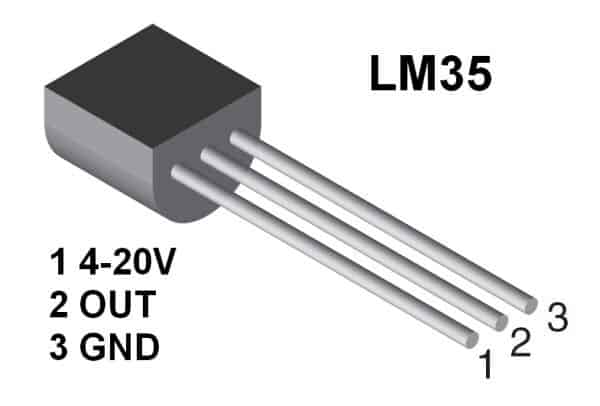
\includegraphics[width=8cm]{lm35.png}
    \caption{پین های سنسور}
    \label{fig:lm35}
\end{figure}
\newline

\newline
\begin{figure}[h]
    \centering
    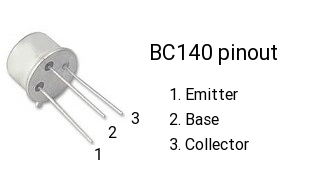
\includegraphics[width=8cm]{bc140.png}
    \caption{پین های ترانزیستور. زائده‌ای که روی ترانزیستور قرار دارد جهت پایه امیتر را نشان می‌دهد.}
    \label{fig:lm35}
\end{figure}
\newline

\newline
\begin{figure}[h]
    \centering
    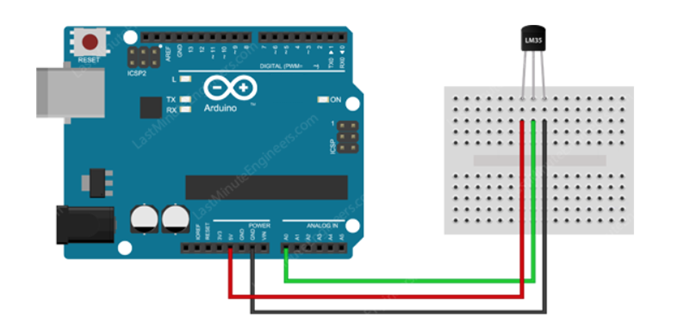
\includegraphics[width=8cm]{l5_c1.png}
    \caption{مدار اتصال سنسور به تنهایی}
    \label{fig:l5-c2}
\end{figure}
\newline

\newline
\begin{figure}[h]
    \centering
    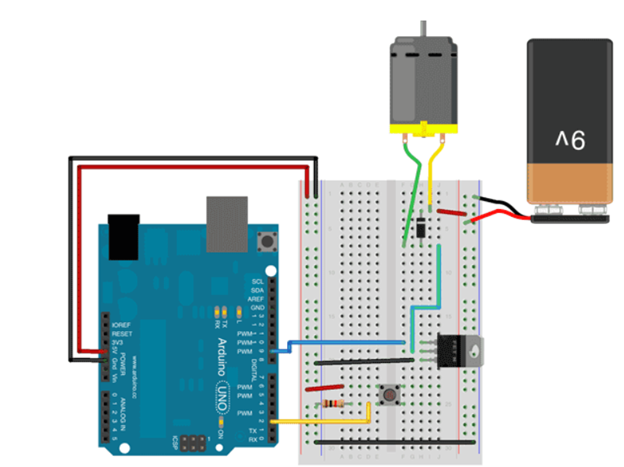
\includegraphics[width=8cm]{l5-c2.png}
    \caption{مدار اتصال موتور. توجه داشته باشید که به جای باطری از منبع تغذیه استفاده می‌کنیم و مقاومت پایه‌ بیس در شکل نیامده. به هیچ عنوان بدون مقاومت متصل به پایه بیس ترانزیستور مدار را روشن نکنید.}
    \label{fig:l5-c2}
\end{figure}
\newline
\section{سروو موتور}
\subsection{اهداف آزمایش}
\begin{itemize}
    \item آشنایی با سروو موتور
    \item آشنایی با \lr{PWM}
    \item آشنایی با مقاومت های حساس به نور
\end{itemize}
\subsection{قطعات مورد نیاز}
\begin{itemize}
    \item \lr{Arduino Uno}
    \item سروو موتور
    \item مقاومت حساس به نور (فوتوسل)
    \item مقاومت ۱۰ کیلواهم
\end{itemize}

\subsection{مقدمه}
\begin{nas}سروو موتور \end{nas}
\paragraph{سروو موتور ها یک نوع از موتور های الکتریکی هستند که به جای چرخیدن، خود را در یک زاویه خاص نگه می‌دارند. این نوع موتور ها در رباتیک کاربرد بسیار زیادی دارند. برای مثال در ساخت دست مصنوعی، ربات های مونتاژ و هر جایی که نیاز داریم چیزی را در یک زاویه خاص قرار دهیم می‌توانیم از سروو موتور استفاده کنید.
}
\paragraph{
سروو موتور ها ۳ ورودی دارند، یکی برای \lr{VCC} که معمولا یک سیم قرمز رنگ است، یکی برای \lr{GND} که معمولا قهوه‌ای یا سیاه رنگ است و سیم سوم که ورودی کنترلی را می‌گیرد. ورودی کنترلی سروو موتور به صورت یک سیگنال \lr{PWM} است و با هر چه \lr{Duty Cycle} بیشتر باشد سروو موتور در زاویه بیشتری قرار می‌گیرد.
}

\paragraph{
\textcolor{red}{\begin{nas}سوال: \end{nas}}
دیتاشیت سروو موتور \lr{SG90} را مطالعه کنید و به سوالات زیر پاسخ دهید:
}
\begin{itemize}
    \item دوره تناوب سیگنال \lr{PWM} چند است؟
    \item دامنه حرکتی این موتور ۱۸۰ درجه است. برای حالاتی که سروو موتور وسط، سمت چپ و یا سمت راست است \lr{Duty Cycle} را محاسبه کنید.
\end{itemize}


\paragraph{
\textcolor{red}{\begin{nas}سوال: \end{nas}}
برای کار با سروو موتور از کتاب‌خانه‌ی \lr{Servo.h} استفاده می‌کنیم. در مستندات این کتاب‌خانه تحقیق کنید و در مورد ورودی، خروجی و کارکرد توابع زیر توضیح دهید.
}
\begin{itemize}
    \item \lr{attach()}
    \item \lr{write()}
\end{itemize}

\begin{nas}مقاومت حساس به نور\end{nas}
\newline
مقاومت های حساس به نور یا فوتورزیستور یا فوتوسل نوعی از مقاومت متغیر است که مقدار مقاومت آن نسبت به نوری که به آن تابیده می‌شود تغییر می‌کند. مقاومت یک فوتوسل در تاریکی زیاد و در روشنایی کم می‌شود. برای اتصال آن به آردوینو می‌توانیم از یک مقاومت \lr{Pull Down} استفاده کنیم.
\newline
\textcolor{red}{\begin{nas}سوال: \end{nas}}
مدار زیر را در نظر بگیرید. اگر مقاومت فوتوسل ۱۰۰ اهم باشد ولتاژ خروجی چند است؟ اگر ۱۰۰ کیلواهم باشد چه؟
\newline
\begin{figure}[h]
    \centering
    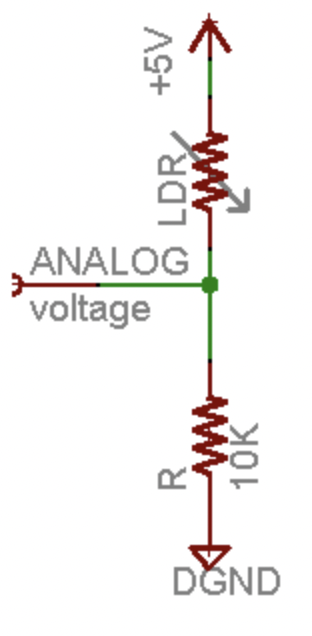
\includegraphics[width=4cm]{ldr-circ.png}
    \caption{مدار اتصال فوتوسل به آردوینو}
    \label{fig:ldr-circ}
\end{figure}
\pagebreak

\subsection{شرح آزمایش}
\begin{enumerate}
    \item فوتوسل را مانند مداری که در مقدمه بررسی کردید به آردوینو متصل کنید. مشخصا باید \lr{Analog Voltage} را به یکی از پین های ورودی آنالوگ متصل کنید.
    \item برنامه‌ای بنویسید که با آن بفهمید خروجی \lr{analogRead} هنگامی که بر روی فوتوسل نور می‌تابد و هنگامی که دستتان را روی آن گرفتید چند است.
    \item سروو را به آردوینو وصل کنید. سیم های \lr{VCC} و \lr{GND} را به ولتاژ ۵ ولت و زمین وصل کنید و سیم کنترلی را به یکی از پین های \lr{PWM} آردوینو. برای این کار می‌توانید از پین های ۹ یا ۱۰ استفاده کنید.
    \item برنامه‌ای بنویسید که ولتاژ فوتوسل را بخواند، اگر مقدار آن ۱۰ درصد کمتر از ولتاژ حالت تاریک باشد زاویه سروو موتور را صفر درجه و اگر مقدار آن ۱۰ درصد بیشتر از ولتاژ حالت روشن باشد زاویه سروو موتور را ۱۸۰ درجه کند. برای این کار می‌توانید از تابع \lr{map} استفاده کنید.
\end{enumerate}
\section{کارگاه اسمبلی اول}

\subsection{اهداف آزمایش}
\begin{itemize}
    \item راه‌اندازی محیط اجرای برنامه های \lr{ARMv7}
    \item آشنایی با قواعد نحوی اسمبلر \lr{GCC}
    \item آشنایی مقدماتی با برنامه نویسی به زبان اسمبلی \lr{ARMv7}
    
\end{itemize}

\subsection{قطعات مورد نیاز}
\begin{itemize}
    \item کامپیوتر متصل به اینترنت و یا کامپیوتری که سیستم عامل لینوکس دارد
\end{itemize}

\subsection{مقدمه}

\paragraph{
همانطور که از اسم درس «آزمایشگاه ریزپردازنده و اسمبلی» پیداست، قسمتی از مباحث ما مربوط به زبان اسمبلی و به طور خاص اسمبلی معماری آرم است.
در کارگاه های آینده زبان اسمبلی را تمرین می‌کنیم و تلاش می‌کنیم که تسلط کافی بر این مبحث داشته باشیم
}

\subsection{راه اندازی محیط اجرا}
\paragraph{
از آنجایی که کامپیوتر های ما معمولا یکی از معماری های
\lr{x86_64}
و 
\lr{ARM64}
هستند باید روشی برای اجرای برنامه های آرم ۳۲ بیتی داشته باشیم. پیشنهاد ما استفاده از
\href
{https://cpulator.01xz.net/?sys=arm}
{
سایت
\lr{CPUlator}
}
است. با استفاده از این سایت می‌توانیم مستقیما برنامه اسمبلی خود را بنویسیم و آن را خط به خط اجرا کنیم و مقادیر رجیستر ها را ببینیم. 
در صورتی که دسترسی به اینترنت ندارید می‌توانید از شبیه‌ساز \lr{QEMU} استفاده کنید اما راه اندازی و استفاده آن مقداری سخت تر است. می‌توانید از این لینک برای آموزش استفاده کنید. توجه کنید که هدف ما آرم ۳۲ بیتی و نه آرم ۶۴ بیتی است.
}

\subsection{آشنایی با قواعد نحوی اسمبلر \lr{GCC}}
\paragraph{
سایت \lr{CPUlator} از اسمبلر \lr{GCC} استفاده می‌کند. در این اسمبلر، نحوه استفاده از دایرکتیو ها مقداری متفاوت از اسمبلر \lr{ARMASM} است که در کلاس تدریس شد. هرچند می‌توانید خودتان برنامه ها را با استفاده از اسمبلر \lr{ARMASM} اسمبل کنید. آموزش انجام این کار را می‌توانید در این لینک ببینید.
}

\paragraph{
خوشبختانه اسامی دستور ها بین این دو اسمبلر یکسان است. تفاوت بزرگ در کدی که می‌نویسید این است که کامنت ها در اسمبلر \lr{GNU} با استفاده از کاراکتر \lr{@} است. همچنین نیازی به \lr{Indentation} صحیح ندارید، اما برای خوانایی کد توصیه می‌شود که آن را رعایت کنید.
}

\subsubsection{لیست دایرکتیو های \lr{GCC} و تفاوت های آن با \lr{ARMASM}}

\begin{itemize}
    \item \lr{.ascii "<string>"} بایت های یک رشته را در برنامه قرار می‌دهند. این دایرکتیو مشابه با دایرکتیو \lr{DCB} است.
    \item \lr{.asciiz "<string>"} مشابه با دایرکتیو \lr{.ascii} با این تفاوت که یک بایت صفر در پایان رشته قرار می‌دهد.
    \item \lr{.byte <byte1>, <byte2>, ...} مشابه با دایرکتیو \lr{DCB}. اسمبلر مقادیر یک بایتی را در برنامه قرار می‌دهد.
    \item \lr{.hword <short1> , <short2>, ...} مشابه با دایرکتیو \lr{DCW}. اسمبلر مقادیر ۲ بایتی را در برنامه قرار می‌دهد.
    \item \lr{.word <word1>, <word2>, ...} مشابه با دایرکتیو \lr{DCD}. اسمبلر مقادیر ۴ بایتی را در برنامه قرار می‌دهد.
    \item \lr{.equ <symbol name>, <value>} مشابه با دایرکتیو \lr{EQU}. اسمبلر یک سمبل تعریف می‌کند و مقدار آن را برابر با مقداری که گذاشتید می‌کند.
    
    \item \lr{.balign <power\_of\_2>{,<fill\_value> ,<max\_padding>} }: آدرس کد یا داده‌ای که پس از این دایرکتیو می‌آید را هم ردیف یک توانی از ۲ می‌کند. برای مثال اگر کد یا داده بعد از آن باید در آدرس ۳ می‌آمد و از اسمبلر خواستیم که آن را هم ردیف ۸ بکند، اسمبلر ۵ بایت اضافه به عنوان \lr{Padding} قبل از آن اضافه می‌کند. این دایرکتیو دو آرگومان اضافه دارد که اولی مقدار بیت های پدینگ را مشخص می‌کند. در صورتی که این آرگومان را نذاشتید بایت صفر به عنوان پدینگ قرار می‌گیرد. آرگومان بعدی حداکثر مقدار بایت های پدینگ را مشخص می‌کند که اگر بایت های پدینگی که باید اضافه می‌شد بیشتر از آن بود اسمبلر کد یا داده بعد از دایرکتیو را هم ردیف نمی‌کند و دایرکتیو بی اثر می‌شود.

\end{itemize}

\subsection{دستور کارگاه}

\paragraph{
همردیف با \lr{n} شدن یعنی اینکه آدرس داده یا کد ما بر \lr{n} بخش‌پذیر باشد. برای مثال همردیف با ۲ یعنی آدرس ما ۰، ۲ ، ۴ و ... باشد. در این کارگاه ابتدا با همردیفی و اهمیت آن و نحوه انجام آن آشنا می‌شویم و سپس یک برنامه ساده برای آشنایی با زبان اسمبلی و نحوه خواندن و نوشتن حافظه در معماری آرم می‌نویسیم.
}

\subsubsection{آشنایی با \lr{alignment} و اهمیت آن}
\begin{itemize}
    \item در بالای کد اسمبلی، رشته \lr{"hello"} را قرار دهید.
    \item بایت های ۱ و ۲ و ۳ را پس از آن قرار دهید.
    \item برنامه را کامپایل کنید و ترتیب قرار گیری رشته و بایت ها و آدرس آن ها را در حافظه ببینید.
    \item با استفاده از دایرکتیو \lr{.balign 13} در میان رشته و بایت ها، تلاش کنید که آدرس بایت ۱ هم ردیف با ۱۳ شود.
    \item تلاش کنید کد را کامپایل کنید. دلیل اروری را که می‌گیرید توضیح دهید.
    \item مقدار \lr{.balign} را به ۴ تغییر دهید. و کد را دوباره کامپایل کنید. چه تفاوتی در ترتیب قرار گیری رشته و بایت ها می‌بینید؟
    \item بعد از لیبل \lr{\_start:} کدی بنویسید که مقدار ۲ را درون رجیستر \lr{r0} قرار دهد و سپس \lr{r0} را با \lr{r0} جمع کند و درون \lr{r1} قرار دهید.
    \item اگر کد را کامپایل کنید هنگام اجرا به یک ارور برخواهید خورد. دلیل این ارور چیست؟
    \item برای حل این مشکل، شروع کدی که نوشتید را هم ردیف با ۴ کنید. کد را دوباره اجرا کنید و با مشاهده مقدار رجیستر ها در اجرای خط به خط برنامه، تایید کنید که همان اتفاقی می‌افتد که می‌خواستیم.
\end{itemize}

\subsubsection{نوشتن یک برنامه ساده اسمبلی}
در این قسمت می‌خواهیم رشته \lr{"hello"} را به \lr{"HELLO"} تغییر بدهیم. در این قسمت از حلقه استفاده نخواهیم کرد و صرفا کد را تکرار می‌کنیم.
\begin{itemize}
    \item ابتدا باید آدرس شروع رشته را بدانیم. برای این کار باید از لیبل ها استفاده کنیم. یکی از لیبل هایی که در کد شما وجود دارد لیبل \lr{\_start:} است. هنگامی که برنامه اسمبل و لینک می‌شود آدرس شروع اجرای برنامه برابر با آدرسی که لیبل \lr{\_start} نشان می‌دهد می‌شود.
    \item لیبل ها در زبان اسمبلی آرم، یک اسم هستند که پس آن : می‌آید. اسمبلر در هنگام اسمبل کردن برنامه شما هر جا که لیبل را دید با آدرس کد یا داده‌ای که پس از لیبل آمده جایگزین می‌کند. برای مثال برای اینکه بخواهیم آدرس شروع رشته را بدانیم کافیست قبل از تعریف رشته یک لیبل اضافه کنیم. این کار را با اسم دلخواه خود انجام بدهید.
    \item برنامه ما باید کاراکتر های رشته را تک تک از حافظه بخواند، مقدار آن را تغییر دهد و مقدار تغییر یافته را در همان آدرس حافظه دوباره بنویسد.
    \item برای خواندن از حافظه، ابتدا باید آدرس لیبل را درون رجیستر \lr{r0} یا هر رجیستر دیگری که می‌خواهید قرار دهید. برای این کار می‌توانید از دستور \lr{MOV} استفاده کنید.
    \item با استفاده از دستور \lr{LDRB} خانه‌ای از حافظه که آدرس آن را \lr{r0} قرار دارد را در \lr{r1} قرار دهید.
    \item برای تبدیل کاراکتر کوچک اسکی به کاراکتر بزرگ، کافیست ۳۲ تا از مقدار کاراکتر کم کنیم. این کار را با استفاده از دستورات جمع و یا تفریق انجام بدهید.
    \item حال باید کاراکتر را در حافظه بنویسیم. آدرس حافظه همچنان در \lr{r0} قرار دارد و کاراکتر تبدیل یافته نیز در \lr{r1} است. با استفاده از دستور \lr{STRB} کاراکتر تبدیل یافته را در حافظه بنویسید.
    \item حال سراغ کاراکتر بعدی می‌رویم. آدرس کاراکتر بعدی یکی از آدرسی که در \lr{r0} قرار دارد بیشتر است، پس کافیست یکی به \lr{r0} اضافه کنیم و مراحل قبل را تکرار کنیم.
    \item این کار را برای هر ۵ کاراکتر رشته تکرار کنید.
    \item برنامه را اجرا کنید و با مشاهده مقادیر رجیستر ها و خانه های حافظه، تایید کنید که برنامه درست کار می‌کند.
\end{itemize}
\section{کارگاه اسمبلی دوم}

\subsection{اهداف آزمایش}
\begin{itemize}
    \item آشنایی با نحوه نوشتن شرط و حلقه در زبان اسمبلی
    
\end{itemize}

\subsection{قطعات مورد نیاز}
\begin{itemize}
    \item کامپیوتر متصل به اینترنت و یا کامپیوتری که سیستم عامل لینوکس دارد
\end{itemize}

\subsection{مقدمه}

\paragraph{
یکی از ساختار هایی که در زبان های برنامه‌نویسی وجود دارد، اجرای شرطی و حلقه ها هستند. پیاده سازی این ساختار ها در زبان اسمبلی نیاز به تمرین دارد و در این کارگاه سعی می‌کنیم با این ساختار ها آشناتر شویم.
}

\subsection{دستور کارگاه}

\subsubsection{آشنایی با نوشتن شرط در زبان اسمبلی}
\begin{itemize}
    \item با استفاده از دستور \lr{B} می‌توانیم به یک قسمت دیگر از برنامه برویم. با استفاده از لیبل ها، برنامه‌ای دلخواه بنویسید که شامل ۵ دستور باشد، اما با گذاشتن دستور \lr{B} بعد از اجرای دستور دوم از دستور های سوم و چهارم پرش شود و دستور پنجم اجرا شود.
    \item حال بالای دستور پرش یک دستور جمع قرار دهید که نتیجه آن برابر با صفر شود.
    \item دستور پرش را به گونه‌ای تغییر دهید که فقط اگر نتیجه دستور قبل بزرگتر (نه بزرگتر‌ مساوی) از صفر بود پرش انجام شود. برنامه خود را اجرا کنید و نتیجه را مشاهده کنید.
    \item دستور جمعی که نوشته بودید را به گونه‌ای تغییر دهید که نتیجه برابر با صفر شود و دوباره نتیجه را مشاهده کنید.
\end{itemize}

\pagebreak

قطعه کد های زیر را مشاهده کنید که کد سی یک دستور شرطی و اسمبلی آن است که توسط کامپایلر ایجاد شده. توجه کنید که کد تولید شده بهینه نیست و می توان چند تا از دستور ها را حذف کرد.
\begin{latin}
\begin{lstlisting}
void compare(int a, int b) {
    if (a > b)
    {
        doIf();
    }
    else
    {
        doElse();
    }
}
\end{lstlisting}
\end{latin}

\begin{latin}
\begin{lstlisting}
        cmp     r0, r1
        ble     .ELSE_TRUE
        b       IF_TRUE
.IF_TRUE:
        bl      doIf()
        b       .POST_IF
.ELSE_TRUE:
        bl      doElse()
        b       .POST_IF
.POST_IF:
\end{lstlisting}
\end{latin}

به طور مشابه کدی بنویسید که دستور شرطی زیر را اجرا کند:
\begin{latin}
\begin{lstlisting}
    if(r0 <= r1) r0 = 0;
    else r0 = 1;
}
\end{lstlisting}
\end{latin}

\subsubsection{آشنایی با نوشتن حلقه در زبان اسمبلی}

\begin{itemize}
    \item با استفاده از دستور برنچ، یک حلقه بی‌نهایت ایجاد کنید که در آن دائما یکی به مقدار رجیستر صفر اضافه می‌شود.
    \item دستور برنچ را به گونه‌ای تغییر دهید که هنگامی که رجیستر صفر به مقدار ۱۰ رسید دیگر حلقه تکرار نشود.
    \item مقدار اولیه رجیستر صفر را قبل از اجرای حلقه به مقدار ۵ تغییر دهید.
    \item حلقه زیر را به زبان اسمبلی بنویسید
\end{itemize}

\begin{latin}
\begin{lstlisting}
for(r0 = 3, r0 < 15; r0 += 2)
{
    r1 += 1;
}
\end{lstlisting}
\end{latin}

\subsubsection{نوشتن یک برنامه کمی پیچیده‌تر اسمبلی}

می‌خواهیم برنامه‌ای که در کارگاه قبل نوشتیم را کمی پیشرفته تر کنیم. یک رشته دلخواه شامل حروف کوچک و بزرگ را در بالای برنامه خود قرار دهید و با استفاده از حلقه و شروط برنامه‌ای بنویسید که حروف کوچک رشته را به حروف بزرگ و حروف بزرگ رشته را به حروف کوچک تبدیل کند. اندازه رشته را می‌توانید به صورت هاردکود شده در برنامه داشته باشید، یا اینکه با استفا
\section{کارگاه اسمبلی سوم}

\subsection{اهداف آزمایش}
\begin{itemize}
    \item آشنایی با نحوه تعریف و کار با ساختار ها در زبان اسمبلی
    \item آشنایی با نحوه تعریف و کار با توابع در زبان اسمبلی
    \item آشنایی با مفهوم \lr{ABI} و لزوم استفاده از آن
\end{itemize}

\subsection{قطعات مورد نیاز}
\begin{itemize}
    \item کامپیوتر متصل به اینترنت و یا کامپیوتری که سیستم عامل لینوکس دارد
\end{itemize}

\subsection{مقدمه}

\paragraph{
در ادامه آشنایی با برنامه‌نویسی به زبان اسمبلی، با ساختار ها و توابع در زبان اسمبلی آشنا خواهیم شد. از آنجا که در اسمبلی صرفا با بایت ها و آدرس ها کار داریم و مفاهیمی مانند تابع و ساختار اساسا وجود ندارند، باید با قواعدی که کامپایلر ها برای پیاده‌سازی این تعاریف استفاده می‌کنند آشنا شویم. این قواعد قسمتی از چیزی هستند که به آن \lr{Appication Binary Interface} گفته می‌شود.
}

\subsubsection{آشنایی با نحوه تعریف و کار با ساختار ها در زبان اسمبلی}

\paragraph{
ساختار یا استراکت یک مفهوم در برخی زبان‌های برنامه نویسی سطح بالا بود که در آن برخی اطلاعات مرتبط به هم را در کنار یک دیگر نگه می‌داشتیم. در زبان اسمبلی ما با بایت ها سر و کار داریم و همانطور که در کارگاه اول دیدیم، هر گاه می‌خواستیم \lr{n} بایت داده بخوانیم، باید آدرس داده‌ها هم‌ردیف با \lr{n} باشد. این مسئله در واقع دلیل قواعد مربوط به چینش استراکت در زبان \lr{C} بود که با آن در درس مبانی برنامه‌نویسی آشنا شدید.
}

\paragraph{برای یادآوری، و همچنین برای استفاده مجدد، این قواعد را در اینجا بازگو می‌کنیم:}

\begin{itemize}
    \item هر فیلد از استراکت، هم‌ردیف با اندازه خودش است.
    \item اندازه کل یک استراکت مضربی از اندازه بزرگ‌ترین فیلد آن است.
    
\end{itemize}

\subsubsection{آشنایی با نحوه تعریف و کار با توابع در زبان اسمبلی}

\paragraph{مانند بقیه چیزهایی که در زبان‌های برنامه‌نویسی سطح بالا داشتیم، تابع نیز در زبان اسمبلی وجود ندارد. در واقع ما در زبان اسمبلی تنها روشی که برای تغییر روند اجرای کد داریم برنچ است. برای اینکه بدانیم توابع سطح بالا پس از کامپایل چه فرمی دارند تا ما نیز از همان فرم استفاده کنیم باید با قواعد مربوطه آشنا شویم. قواعد اصلی آن در کلاس درس به عنوان استاندارد \lr{AAPCS} معرفی شد. در کارگاه از یک نسخه ساده‌سازی شده این قواعد استفاده خواهیم کرد.}

\paragraph{
نکته اصلی قاعده مربوط به صدا زدن توابع این است که ما رجییستر ها را به دو بخش تقسیم می‌کنیم، رجیستر هایی که حفظ آن‌ها وظیفه صدا زننده تابع است، و رجیستر هایی که حفظ آن‌ها وظیفه تابع صدا زده شده است. برای مثال اگر بگوییم \lr{r0} را صدا زننده حفظ کند و \lr{r1} را صدا زده شده، برنامه ما قبل از صدا زدن تابع باید \lr{r0} را در استک قرار دهد و تابع نیز اگر از \lr{r1} استفاده می‌کند باید آن‌را در استک قرار دهد و قبل از پایان تابع مقدار اصلی آن‌را باز گرداند.
}

\paragraph{در این کارگاه قرارداد می‌کنیم که رجیسترهای صفر تا سوم را صدا زننده تابع حفظ کند، و رجیستر های چهارم تا دوازدهم به علاوه رجیستر \lr{lr} را تابع صدا زده شده حفظ کند. باقی رجیسترها خاص منظوره‌اند و نباید از آن‌ها استفاده کنید. برای هر کدام از توابع خود باید یک لیبل بگذارید و صدا زدن تابع نیز با استفاده از دستور \lr{bl} و برگشتن از تابع با استفاده از دستور \lr{bx lr} صورت می‌گیرد.}

\paragraph{اما آرگومان های ورودی توابع چگونه به ورودی داده می‌شوند؟ این نیز در استاندارد \lr{AAPCS} گفته شده. در این کارگاه قرارداد می‌کنیم که از رجیستر های صفر تا چهارم برای ورودی‌ها استفاده کنیم. مقدار خروجی نیز در رجیستر صفر قرار می‌گیرد.}

\paragraph{
در نتیجه برای توابع باید نکات زیر را رعایت کنید:
}
\begin{itemize}
    \item برای صدا زدن تابع ابتدا رجیستر های صفر تا سه را در استک حفظ کنید، سپس آرگومان های ورودی را به ترتیب در رجیستر های صفر تا سه قرار دهید، تابع را صدا بزنید، مقدار خروجی تابع را نگه‌دارید و سپس رجیستر صفر تا سوم را از استک برگردانید.
    \item تابعی که صدا زده می‌شود حق دارد بدون حفظ کردن در استک از رجیستر های صفر تا سه استفاده کند.
    \item تابعی که صدا زده می‌شود باید رجیستر \lr{lr} را ابتدای تابع در استک حفظ کند و قبل از بازگشت از تابع آن را از استک برگرداند.
    \item در صورتی که از رجیستر های چهارم تا دوازدهم در تابع استفاده شد، تابع باید آن‌ها را ابتدای اجرا در استک حفظ کند و قبل از بازگشت از تابع آن ها را از استک برگرداند.
\end{itemize}

\subsection{دستور کارگاه}


\begin{itemize}
    \item یک تابع برای به توان دو رساندن بنویسید و با استفاده از قراردادی که داشتیم، آن را به درستی صدا بزنید.
    \item یک تابع بازگشتی بنویسید که یک عدد \lr{n} به عنوان ورودی بگیرد و عدد \lr{n}ام فیبوناچی را در خروجی بازگرداند.
    \item در فایل 
    \lr{data.asm}
    یک درخت با شما داده شده است که ۴ بایت اول آن مقدار داده درخت، ۴ بایت بعدی فرزند راست و ۴ بایت بعدی فرزند چپ درخت است. با دایرکتیو 
    \lr{.space <number\_of\_bytes>}
    هفت ورد فضا رزرو کنید، به صورت 
    \lr{Post-Order}
    در درخت پیمایش کنید و مقادیر گره های درخت را در فضایی که رزرو کردید بنویسید.
\end{itemize}


کد پیمایش درخت:
\begin{latin}
\begin{lstlisting}
struct tree{
    int val;
    struct tree *right;
    struct tree *left;
}
void post_order(struct tree *root){
    if(root == 0) return;
    post_order(root->left);
    post_order(root_right);
    print(root->val); //store in reserved space instead of printing
}
\end{lstlisting}
\end{latin}
\end{document}